%% Use the standard UP-methodology class
%% with French language.
%%
%% You may specify the option 'twoside' or 'oneside' for
%% the document.
%%
%% See the documentation tex-upmethodology on
%% http://www.arakhne.org/tex-upmethodology/
%% for details about the macros that are provided by the class and
%% to obtain the list of the packages that are already included. 
 
\documentclass[english]{spimubphdthesis}
 
%%--------------------
%% The TeX code is entering with UTF8
%% character encoding (Linux and MacOS standards)
\usepackage[utf8]{inputenc}
 
%%-------------------
%% You want to use the NatBib extension
%\usepackage[authoryear]{natbib}
 
%%--------------------
%% Include the 'multibib' package to enable to
%% have different types of bibliographies in the
%% document (see at the end of this template for
%% an example with a personnal bibliography and
%% a general bibliography)
%%
%% Each bibliography defined with 'multibib'
%% adds a chapter with the corresponding
%% publications (in addition to the chapter for
%% the standard/general bibliography).
%% CAUTION:
%% There is no standard way to do include this type of
%% personnal bibliography.
%% We propose to use 'multibib' package to help you,
%% for example.
%\usepackage{multibib}
 
%% Define a "type" of bibliography, here the PERSONAL one,
%% that is supported by 'multibib'.
%\newcites{PERSO}{Liste de mes publications}
 
%% To cite one of your PERSONAL papers with the style
%% of the PERSONAL bibliography: \citePERSO{key}
%% To force to show one of your PERSONAL papers into
%% the PERSONAL bibliography, even if not cited in the
%% text: \nocitePERSO{key}
 
%% REMARK: When you are using 'multibib', you
%% must compile the PERSONAL bibliography by hand.
%% For example, the sequence of commands to run
%% when you had defined the bibliography PERSO is:
%%   $ pdflatex my_document.tex
%%   $ bibtex my_document.aux
%%   $ bibtex PERSO.aux
%%   $ pdflatex my_document.tex
%%   $ pdflatex my_document.tex
%%   $ pdflatex my_document.tex
 
%%--------------------
%% Add here any other packages that are needed for your document.
%\usepackage{eurosim}
%\usepackage{amsmath}

%% Rick add usepackage
%%
%\usepackage{graphicx}
%\usepackage{epsfig}
%\usepackage{mathrsfs}
%\usepackage{times}
%\usepackage{makeidx}
\usepackage{amsmath}
%\usepackage{algorithm}
%\usepackage{algorithmic}
%\usepackage{booktabs}
%\usepackage[flushleft]{threeparttable} % http://ctan.org/pkg/threeparttable
%\usepackage{multicol}
%\usepackage{array}
%\usepackage[binary-units=true]{siunitx}
%\usepackage{balance} % This allows for the even columns in the final page, just insert \balance in the last page, e.g., before the reference list
%\usepackage{cite}
 
%%--------------------
%% Set the title, subtitle, defense date, and
%% the registration number of the PhD thesis.
%% The optional parameter is the subtitle of the PhD thesis.
%% The first mandatory parameter is the title of the PhD thesis.
%% The second mandatory parameter is the date of the PhD defense.
%% The third mandatory parameter is the location/city of the PhD defense.
%% The forth mandatory parameter is the reference number given by
%% the University Library after the PhD defense.
\declarethesis[This is the sub-title]{Performance Estimation, Testing, and Control of Cyber-Physical Systems Employing Non-Ideal Communications Networks}{9 July 2020}{Dijon}{XXX}
 
%%--------------------
%% Set the author of the PhD thesis
\addauthor[email]{Richard}{Candell}
 
%%--------------------
%% Add a member of the jury
%%
%% CAUTION 1: If a Jury member is not present during the defense,
%%            she/he must be in the list of the Jury members.
%%            Only the reviewers and the members who are present during the defense must
%%            appear in the Jyry member list. 
%% CAUTION 2: After your defense, you must assign the role "Pr\'esident" to
%%            the Jury member who have been the President of the Jury.
%% CAUTION 3: The recommended order for the Jury members is:
%%            President, Reviewer(s), Examiner(s), Director(s),
%%            Other supervisor(s), Invited person(s).
%% \addjury{Firstname}{Lastname}{Role in the jury}{Position}
\addjury{Incroyable}{Hulk}{Pr\'esident}{Professeur à l'Université de Gotham City \\ Commentaire secondaire}
\addjury{Captain}{America}{Rapporteur}{Professeur à l'Université USA}
\addjury{Super}{Man}{Examinateur}{Professeur à l'Université de Gotham City}
\addjury{Bat}{Man}{Directeur de thèse}{Professeur à l'Université de Gotham City}
\addjury{The}{Volwerine}{Codirecteur de thèse}{Professeur à l'Université de Gotham City}
\addjury{Pac}{Man}{Invité}{Professeur quelque part}
 
%%--------------------
%% Change style of the table of the jury
%% \Set{jurystyle}{put macros for the style}
%\Set{jurystyle}{\small}
 
%%--------------------
%% Set the English abstract
\thesisabstract[english]{Lorem ipsum dolor sit amet, saepe quodsi dolores an usu. An sed fugit dissentiunt, ex tota soleat duo. Omnes deserunt adversarium qui ad, periculis pertinacia has id. Ea tibique antiopam eos. Usu illud cetero voluptatum ne, ea odio soluta labores sit.	Pri modus eruditi definiebas an. Dicat latine inermis no quo, eos tollit delicata interesset cu. Placerat vituperatoribus pro ne, cu verear tritani deterruisset usu. Quaeque recusabo maluisset te pri, mutat maiorum accusamus at his.	Pro ad nihil deleniti senserit, mundi feugiat indoctum an sea. In consulatu efficiendi qui, eu duo dicta deserunt definitiones, te atqui sapientem adolescens sit. Id pro consulatu splendide evertitur, vis eu perpetua molestiae, an melius virtute efficiantur vis. Animal aeterno mei ei.	Lucilius suavitate euripidis vis id, cu dicam ridens forensibus vis. In incorrupte adversarium pri, ut velit singulis nec, nisl facer dissentias ex duo. Id est nulla periculis, epicuri percipit cu eum. Praesent temporibus mediocritatem ex cum, his quot nonumy iriure ut, qui natum aliquip id. Interesset quaerendum repudiandae cum ea. Mazim perpetua deterruisset ne mei, cum esse novum minimum ea.}
 
%%--------------------
%% Set the English keywords. They only appear if
%% there is an English abstract
\thesiskeywords[english]{industrial wireless, factory communications, networked control, manufacturing}
 
%%--------------------
%% Set the French abstract
\thesisabstract[french]{Lorem ipsum dolor sit amet, saepe quodsi dolores an usu. An sed fugit dissentiunt, ex tota soleat duo. Omnes deserunt adversarium qui ad, periculis pertinacia has id. Ea tibique antiopam eos. Usu illud cetero voluptatum ne, ea odio soluta labores sit.	Pri modus eruditi definiebas an. Dicat latine inermis no quo, eos tollit delicata interesset cu. Placerat vituperatoribus pro ne, cu verear tritani deterruisset usu. Quaeque recusabo maluisset te pri, mutat maiorum accusamus at his.	Pro ad nihil deleniti senserit, mundi feugiat indoctum an sea. In consulatu efficiendi qui, eu duo dicta deserunt definitiones, te atqui sapientem adolescens sit. Id pro consulatu splendide evertitur, vis eu perpetua molestiae, an melius virtute efficiantur vis. Animal aeterno mei ei.	Lucilius suavitate euripidis vis id, cu dicam ridens forensibus vis. In incorrupte adversarium pri, ut velit singulis nec, nisl facer dissentias ex duo. Id est nulla periculis, epicuri percipit cu eum. Praesent temporibus mediocritatem ex cum, his quot nonumy iriure ut, qui natum aliquip id. Interesset quaerendum repudiandae cum ea. Mazim perpetua deterruisset ne mei, cum esse novum minimum ea.}

 
%%--------------------
%% Set the French keywords. They only appear if
%% there is an French abstract
\thesiskeywords[french]{Mot-cl\'e 1, Mot-cl\'e 2}
 
%%--------------------
%% Change the layout and the style of the text of the "primary" abstract.
%% If your document is written in French, the primary abstract is in French,
%% otherwise it is in English.
%\Set{primaryabstractstyle}{\tiny}
 
%%--------------------
%% Change the layout and the style of the text of the "secondary" abstract.
%% If your document is written in French, the secondary abstract is in English,
%% otherwise it is in French.
%\Set{secondaryabstractstyle}{\tiny}
 
%%--------------------
%% Change the layout and the style of the text of the "primary" keywords.
%% If your document is written in French, the primary keywords are in French,
%% otherwise they are in English.
%\Set{primarykeywordstyle}{\tiny}
 
%%--------------------
%% Change the layout and the style of the text of the "secondary" keywords.
%% If your document is written in French, the secondary keywords are in English,
%% otherwise they are in French.
%\Set{secondarykeywordstyle}{\tiny}
 
%%--------------------
%% Change the speciality of the PhD thesis
\Set{speciality}{Informatique}
 
%%--------------------
%% Change the institution
\Set{universityname}{Universit\'e de Bourgogne}
 

%%--------------------
%% Clear the list of the laboratories
\resetlaboratories

%%--------------------
%% Add the laboratory where the thesis was made
%\addlaboratory{Laboratoire Waynes Industry}

\addlaboratory{Laboratoire \'Electronique, Informatique et Image}


%%--------------------
%% Clear the list of the partner/sponsor logos
%\resetpartners

%%--------------------
%% Add the logos of the partners or the sponsors on the front page
%%
%% CAUTION 1: At least, the logo of the University should appear (UB)
%%
%\addpartner[image options]{image name}

%\addpartner{ub}

%%--------------------
%% Change the header and the foot of the pages.
%% You must include the package "fancyhdr" to
%% have access to these macros.
%% Left header
%\lhead{}
%% Center header
%\chead{}
%% Right header
%\rhead{}
%% Left footer
%\lfoot{}
%% Center footer
%\cfoot{}
%% Right footer
%\rfoot{}
 
%%--------------------
% Declare several theorems
\declareupmtheorem{mytheorem}{My Theorem}{List of my Theorems}

%%--------------------
%% Change the message on the backcover.
%\Set{backcovermessage}{%
%	Some text
%}

\begin{document}
 
%%--------------------
%% The following line does nothing until
%% the class option 'nofrontmatter' is given.
%\frontmatter

%%--------------------
%% The following line permits to add a chapter for "acknowledgements"
%% at the beginning of the document. This chapter has not a chapter
%% number (using the "star-ed" version of \chapter) to prevent it to
%% be in the table of contents
\chapter*{Acknowledgments}
The author would like express his gratitude to his beautiful daughter, Erin, for all of her generous support and care during a very trying time.

Other acknowledgements: Mohammed, Yongkang, Karl




 
%%--------------------
%% Include a general table of contents
\tableofcontents

%%--------------------
%% The content of the PhD thesis
\mainmatter
 
\part{Context and Problem Statement}

\chapter{Introduction}

\section{Industrial Revolutions}
Major advances in manufacturing of goods for the betterment of humanity have occurred many times in the last two hundred and fifty years in the history of humanity.  These advancements occurred of science and technology occurred as revolutionary events at different times.  The first revolution occurred at the edge of the eightieth century primarily in England but also in France, Germany, and the United States with the applicant of automatic mechanization of large machines using coal powered steam engines.  These machines were mainly used for the processing of cotton, wool, and silks in the production of textiles for export throughout the world.  Advancements during this period included uses of coal to produce steam power, the production of iron, steel, and other rudimentary alloys, and, very importantly, the engineering advancements of tool making.  The advancements of the first industrial revolution paved the way for the centralization and mass production of goods.
%CITATION SOURCES *** {https://en.wikipedia.org/wiki/Technological_revolution#Potential_future_technological_revolutions}

The next century was marked by the development of scientific and engineering advancements in chemistry, physics, and engineering. Experimentation with electricity and the production thereof led to the eventual explosion of industrial machinery, tooling, electrification, chemical manufacture, petroleum refinement, rail and marine transportation, the automobile, agriculture, and telecommunications by wire over long distances.  This period of discovery culminated with rapid expansion of industrialization through the world, especially in North America and Japan up until the beginning of World War I.
%CITATION SOURCES *** https://en.wikipedia.org/wiki/Second_Industrial_Revolution#Machine_tools

The third industrial revolution began in the tears immediately following the second world war with the rapid advancement of pure and applied sciences.  These advancements were driven primarily by the cold war and the space race between the United States and the USSR.  This period of advancement was marked by many discoveries and scientific applications such as the development of telecommunications theories (Claude Shannon), advancement of radio and wired communications, the discovery of the transistor, and the rapid expansion of computers and information technology in business and defense.  Also during these years, arrived the application of computing within manufacturing and process control settings. Computers slowly began to replace the basic relay circuit in control systems.  By utilizing the programmable logic controller (PLC), manufacturers gained the ability to develop control their processes more easily and develop control strategies that were once more difficult to implement in the past with dedicated, specialized equipment.  PLCs offered both the ability to more easily adapt processes to information gathered directly from the factory operation as well as slowly collect and store information electronically.  However, electronic storage of this information was still both difficult and expensive as telecommunications technology was yet relatively slow and storage expensive.  Over the years following through the 1980's until today, computers have followed closely Moore's "Law" which states according to the the perception of Intel Corporation founder, Gordon E. Moore, that the number of transistors on a microchip doubles every two years.  This paradigm of exponential growth in digital computing technology in terms of computing speed, storage, and efficiency has created a world in which computers and computing devices have become ubiquitous, surrounding practically every aspect of human endeavours and leading to the latest installment of industrial advancement, the 4\textsuperscript{th} Industrial Revolution, also known as the \textit{Information Revolution} which is currently ongoing. 

The Information Revolution is defined by a culture that is highly interconnected and data depended.  Clearly, the modern world is dominated by the Internet, high-performance computers, and personal mobile communications devices such as cell phones developed over the last several decades. Within the hands of each individual one may find a smartphone capable of performing computing and communications tasks not even imaginable fifty years ago.  Indeed, within each of these devices resides a powerful microprocessor capable of clocking speeds in the gigahertz, offline storage spanning gigabytes, at-least one high-resolution camera, and communication components enabling high-speed connectivity capable.  These personal devices are smart and easily re-programmable by downloading of new applications, i.e., \textit{apps} enabling users to produce and consume information rapidly.  Users enjoy the ability to speak at any moment, send brief messages using apps such as WhatsApp\texttrademark, download videos, play games, store documents, music, photographs, and videos within "the cloud."  Within office and business enterprises, a personal computer is within reach of every employee and is the tool used for information production.  The data produced is stored within the cloud and usually produced and maintained locally, although the services of data production are quickly shifting to the cloud as well depending on the needs the end user.

These capabilities have also been permeating industrial environments although at a slower rate given the inherent conservatism of industrial establishments.  Industrial environments include aerospace and automotive manufacturing, electrical power production, food processing, petroleum and chemical production.  That is not to say that industrial establishments are not open to technological change, but that established production system can be difficult or risky to modify once they are operational.  While industrial operations have distinctly different requirements than office businesses; analogues may be made between the computing constructs found within the personal/business computing domains and those constructs founds within the industrial computing domains.  For example, within a factory production enterprise, the Internet itself exists as an outside entity providing global connectivity, hosting, storage, computing resource, and analysis tools.  These services are often replicated within the business enterprise of the factory operation and extended into the factory environment to some degree from the factory management system to the factory floor.  

In addition, with the explosiveness of ubiquitous, low-cost computing devices, the modern factory operation is changing to include more intelligence and adaptability at the factory edge.  This includes discrete devices such as sensors and actuators, collaborative robots, autonomous gantry systems, intelligent vehicular systems, tracking and inventory systems, and the like.  These systems coupled with the plethora of computing resources have the potential to create an enormous amount of information as well as the opportunities for greater control over the factory enterprise.  It is just a matter of tapping the information within the factory and bringing that information to a useful purpose.  Where the third industrial revolution brought computing and automation to the factory, the fourth industrial revolution will improve upon the automation found within the factory by adding intelligence, autonomy, and machine learning powered by data. This defines Industry 4.0.  

\section{Industry 4.0}

Industry 4.0 also known as "smart manufacturing" was officially launch by President Barack Obama of the United States and Chancellor Angela Merkel of Germany at the Hannover Messe industry show on April 24, 2016\textcolor{red}{\cite{DUMMY01}}.  Smart manufacturing is a term used to described the ongoing efforts within academia, government, and private industry to improve upon existing and future factory operations by incorating

\begin{figure}[!tbp]
	\begin{center}
		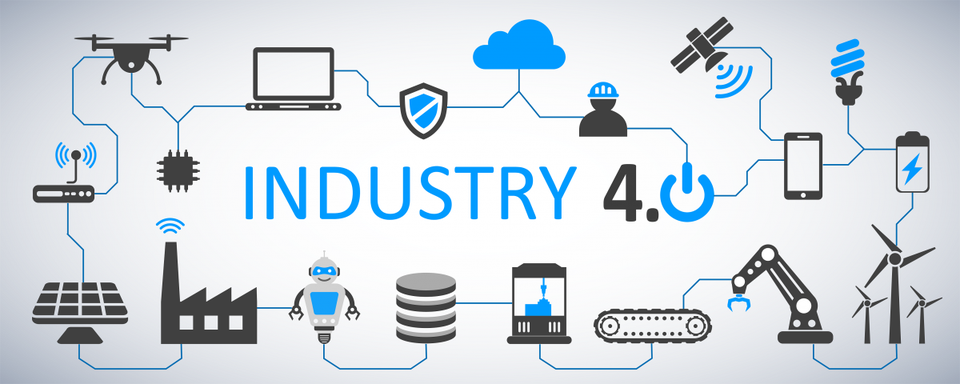
\includegraphics[width=\textwidth]{images/intro/forbes-i40.png}
		\label{fig:intro:forbes-i40}
		\caption{Industry 4.0: Incorporating the benefits of machine learning, massive data, mobility, and autonomy within the modern factory.  %https://www.forbes.com/sites/bernardmarr/2018/09/02/what-is-industry-4-0-heres-a-super-easy-explanation-for-anyone/#6dee527a9788}
	\end{center}
\end{figure}

Industry 4.0 is a term used to describe the latest evolution trend in global industrialization with respect to manufacturing.  It is marked by the ambitious end goal of a completely automated and data-driven factory enterprise.  The concept of Industry 4.0 is centered around the smart factory in which . 

Computer

“Industry 4.0” is an abstract and complex term consisting of many components when looking closely into our society and current digital trends. To understand how extensive these components are, here are some contributing digital technologies as examples:[25]

Mobile devices
Internet of Things (IoT) platforms
Location detection technologies
Advanced human-machine interfaces
Authentication and fraud detection
3D printing
Smart sensors
Big data analytics and advanced algorithms
Multilevel customer interaction and customer profiling
Augmented reality/ wearables
Fog, Edge and Cloud computing
Data visualization and triggered "real-time" training
Mainly these technologies can be summarized into four major components, defining the term “Industry 4.0” or “smart factory”:[25]

Cyber-physical systems
IoT
Cloud computing
Cognitive computing

\section{Manufacturing Enterprise}
ISA-95 model of distributed hierarachical: Batch production, Job production, Flow production
Modern paradigms: Edge computing, AI/ML

\begin{figure}[!tbp]
	\begin{center}
		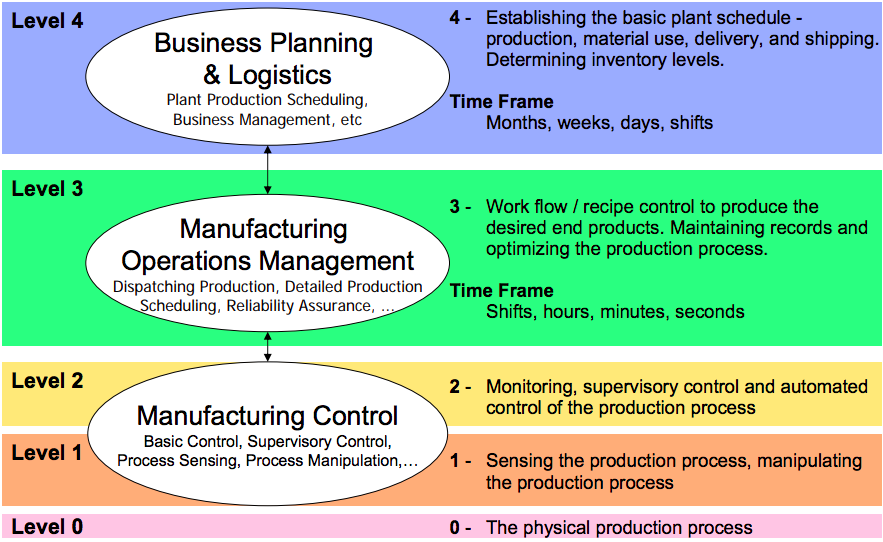
\includegraphics[width=\textwidth]{images/intro/isa95-2.png}
		\label{fig:intro:isa95}
		\caption{The ISA-95 model: Legacy enterprise model developed by the ISA which divides production systems into 5 distinct levels based on the Purdue Enterprise Reference Architecture (PERA).}
	\end{center}
\end{figure}

Unlike the MESA model, which focused on business process, the ISA-95 model focuses on information architecture. The ISA-95 model divides production systems into 5 levels, based on the Purdue Enterprise Reference Architecture (PERA) model.

In this way, the ISA-95 standard helps define boundaries between systems. Intelligent devices, such as sensors, belong to Level 1. Control systems such as PLCs , DCS, OCS, belong to Level 2. MES, belong to Level 3. ERP to level 4.

By situating MES on Level 3, ISA-95 implies that MES connect production with enterprise systems, manage workflows to produce end products, maintain records of production, and optimize the production process.

The goal was to develop a standard that would enable efficient interfacing and integration between an ERP system and an MES. This would facilitate effective communication between stakeholders, lowering the total cost of ownership and enabling error-free integration.


\section{The Importance of Wireless in Automation}

The fourth industrial revolution, commonly referred to as Smart Manufacturing in the U.S. and Industry 4.0 in Europe, promises unparalleled productivity and capability advances in the manufacturing.  Propelled by economic pressure toward greater efficiency, factory agility, and product customization, future factories will have the technological ability to adapt to customer demands quickly, modify manufacturing processes automatically based on quality feedback, and fabricate products with a reduced environmental impact.  Technological advances required for smart manufacturing to be truly successful include a collaborative and mobile robotics, distributed machine autonomy based on artificial intelligence, and a high degree of interconnectivity of among the automation resources.  Robots will work together and with people to accomplish complex tasks.  Robots will have the ability to roam between work-cells within a factory, learn its role quickly, become aware of edge devices, and communicate with other actors within the work-cell to accomplish its goals.  Current manufacturing architectures use wired connectivity through field bus and industrialized Ethernet for sensing and real-time control.  

Indeed, through advances in time-sensitive networking, many of the promises of smart manufacturing are being realized; however, the true goals of smart manufacturing require a large deployment of sensing and actuation devices and untethered (i.e. mobile), autonomous robotics actors.  The use of wires precludes mobility and makes deployment of edge devices more expensive as each devices requires power, wires, and conduit for communication. By adopting wireless for both sensing and control of machines within the work-cell, a lower-cost, untethered operation is achievable. once wireless is adopted as the primary mode of communication, questions arise as to the required latency, reliability, and scale of the wireless network especially when the network is used for the control of machines and the assurance of safety. 

Latency is defined as the data time-of-flight between two applications, e.g. when an event is acquired at a sensor to the point it is made available at a programmable logic controller (PLC).  Reliability is defined as the data loss probability between two applications. Scale is defined as the number of stations accessing the wireless network.  The requirements of reliability, latency, and scale directly relate to the complexity and cost of the wireless network; therefore, a rigorous analysis, validated by physics and untainted by market hype, is necessary to define realistic, achievable, and cost effective performance parameters of the wireless network.  In this paper, we investigate the validity of commonly advertised requirements of wireless networks used for industrial control systems whiling providing a validated perspective on those requirements making realization of such networks more achievable using existing technologies.  We begin with a close examination of existing wireless network requirements for factory automation. We follow with an architectural analysis of the future collaborative work-cell. This architectural analysis drives a cyberphysical system simulation to determine limits of reliability, latency, and scale constraints of wireless stations within the work-cell.  We then conclude with recommendations for reliability, latency, and scale constraints that will accommodate most industrial automation applications and are realizable with devices that are based on ubiquitous standards.

\section{Challenges in Industrial Wireless Networks}

\subsection{Avoiding the Hype: Understand the Requirements}
\subsection{Interference}
\subsection{Multi-path Propagation}
\subsection{Reliability}
\subsection{Latency in Time-sensitive Applications}
\subsection{Energy Efficiency Application for Battery-powered Devices }
\subsection{Trading Reliability, Latency, Scale, and Power}

\subsection{Trade-space for Requirements}
Insert special graph showing the competing requirements

\section{Industrial Wireless Use Cases}

\section{Plethora of Wireless Technologies}
Explain the plethora of wireless tech available, difficulty understanding which if any tech is applicable to a particular use case

Show the resilience week paper

Show 

\section{Need for Evaluation Methods }
Explain how testing the communication network is not sufficient.  need to test the impact of network on the physical system.  Need methods by which to do this.  Start with requirements, proceed to design of the system, and then verification of performance of network AND physical system, and then feedback into design/requirements.

Need to show the architecture

L'objectif principal de votre thèse peut être mis en avant à l'aide de l'environnement ci-dessous:

\begin{emphbox}
	Proposer un modèle qui fait quelque chose!
\end{emphbox}

\chapter{Thesis Summary}

\section{Thesis Objectives}

\section{Thesis Organization}


\part{Technical Contributions}
\chapter{Survey: Industrial Wireless Technology}
reslience week article
\chapter{Guidelines: Industrial Wireless Deployments}
NIST guidelines, industry led forum and results on AMS 300-4
\chapter{Wireless Workcell Architecture}


%
\section{Introduction} \label{sec:intro}    
The fourth industrial revolution promises unparalleled productivity and capability advances in manufacturing. To support the manufacturing industry in this conversion, various programs have been established in several countries such as Smart Manufacturing in the U.S.~\cite{SmartManuf} and Industry 4.0 in Europe~\cite{Industry40, cpsInd4.0}. Propelled by economic pressure toward greater efficiency, factory agility, and product customization, future factories will have the technological ability to adapt to customer demands quickly, modify manufacturing processes automatically based on quality feedback, and fabricate products with a reduced environmental impact.  Technological advances required for smart manufacturing to be successful include collaborative and mobile robotics~\cite{indRobot2017}, distributed machine autonomy based on artificial intelligence \cite{ManufAI2009}, improved process observability~\cite{IIoToverview2018}, and a high degree of interconnectivity among automation resources~\cite{ieMag2018}. Work-cells are self-contained units of operation within a factory~\cite{CHEN2001199, JMarvel2017, 6059204}.  These work-cells are composed of various machines, conveyors, motors, edge devices, and robots.  Robots will work together and with people to accomplish complex tasks or to tending to other machines within the work-cell.  Robots will have the ability to roam between work-cells within a factory, learn their roles quickly, become aware of edge devices, and communicate with other actors within the work-cell to accomplish their goals. Efficient communications between robots and the other players in the work-cell are essential to the fulfillment of the robot-related tasks.

Current manufacturing architectures use wired connections through field-bus and industrial Ethernet protocols for sensing and real-time control~\cite{etherCAT, indPrinter}.  Indeed, through advances in time-sensitive networking, many of the promises of smart manufacturing are being realized; however, the true goals of smart manufacturing require a large deployment of sensing and actuation devices and mobile, perhaps autonomous, robotics actors~\cite{ieMag2018}.  The use of wires precludes mobility and makes deployment of edge devices more expensive as each  requires power, cables, and conduit for communication. By adopting wireless for both sensing and control of machines within the work-cell, a lower-cost, untethered operation is achievable\footnote{The power for untethered operation can be achieved through the use of rechargeable batteries to power the untethered machine or robot for enough operating period.}. Once wireless is adopted as the primary mode of communication, questions arise as to the required latency, reliability, and scale of the wireless network especially when the network is used for the control of machines and the assurance of safety~\cite{ieMag2018}. 

The work presented here addresses the present need for a comprehensive architectural model of the factory work-cell in which wireless is a preferred mechanism for carrying information within the work-cell. We begin with an architectural analysis of the future collaborative work-cell that includes edge devices, robots, vision systems, and supervisory controllers. Our architectural analysis includes structural components, information flows, and parametric elements of the work-cell. We identify factors that limit reliability, latency, and scalability of the wireless network, and we conclude with a discussion of significant information flows. Significant information flows are defined as operationally critical or safety-related.  Our contributions are:

\begin{itemize}
	\item[$\star$] First, we develop a comprehensive and extensible architectural model using the Systems Modeling Language (SysML) that provides primitives for describing the physical and networking components of a work-cell with parametric constraints\footnote{We make the model publicly available for download. A valid license of MagicDraw 18.5 is required to use the model.  A web-based report of the model is provided for read-only access.};
	\item[$\star$] Second, we provide a framework for analyzing cross-domain interactions of complex wireless work-cell deployments; and
	\item[$\star$] Third, significant information flows are identified, annotated with rate constraints.
\end{itemize}

The remainder of this paper is organized as follows:  In Section~\ref{sec:related-work}, previous related work is discussed and our motivation for constructing a model is presented.  A brief introduction to systems modeling is presented in Section~\ref{sec:systemsmodeling} and provides a primer on the SysML language. The conceptual architecture of the model providing a concept-of-usage is proposed in Section~\ref{sec:conceptual}, followed by a detailed exposition of each package in Section~\ref{sec:detailed-model}.  Then, in Section~\ref{sec:wireless-infoflows}, significant information flows are discussed through introducing a case study. Section~\ref{sec:conclusion} concludes the paper and identifies opportunities for future research.

\section{Related Work}\label{sec:related-work}

Current modeling work on factory work-cells is mainly aimed at defining and characterizing the subsystems, such as human staff, robots, and machine tools, in individual applications. By following blueprints (schematics) of production tasks, the work flow can be divided into separate assignments which are distributed by a task dispatch system to individual machines~\cite{IkeaBot}. Analytical models are thus obtained for performance analysis in work-cells. As an example, a mathematical model for real-time performance analysis of a gantry work-cell with robots is established with the timing and the randomness of tasks and disruptions are captured  \cite{8098604}. In \cite{OU2017212}, the same model is used to investigate the system natural properties such the system cycle and waiting times and to identify bottlenecks through studying the sensitivity of each machine. Similarly, the steady state analysis for production lines with uncertainties is performed through various decomposition methods~\cite{Colledani2013,doi:10.1080/00207543.2012.713137,doi:10.1080/00207540500385980}. In \cite{Colledani2013}, a decomposition method is presented for the analysis of continuous flow lines. The presented model is used to analyze flow lines with single and multiple failure mode machines and machines subject to aging and having up and down times. In \cite{doi:10.1080/00207543.2012.713137}, a model to evaluate the performance of transfer lines with unreliable machines and finite transfer-delay buffers is presented. A decomposition method is introduced to model the transfer line, using the general-exponential distributions instead of the exponential distributions to approximate the repair time distributions of the fictitious machines. In \cite{doi:10.1080/00207540500385980}, the authors present a model for evaluating the production rate and distribution of inventory of a closed-loop manufacturing system with unreliable machines and finite buffers. The model accounts for the different sets of machines that could cause blockage or starvation to other machines. In \cite{QChang,Liu2012}, the performance analysis modeling for serial production lines with disruptions is explored by studying the impact of each individual downtime event in terms of permanent production loss and financial cost. These analytical models generally work well for simple systems with small number of components or few interactions between various equipment. Also, the analytical models can be used to abstract industrial systems to understand various performance trends without studying various details. As a result, we introduce a comprehensive model that include network and production impacts on the industrial work-cell.  

Furthermore, the reconfigurable work-cell architecture is widely considered for automated manufacturing. The main advantage of reconfigurable work-cells lies in the flexibility of reconfiguration of work-cell components to adapt to varying production requirements where the assembly of the work cell is optimized for each specific task~\cite{CHEN2001199}. In the work-cell that hosts robots, robots are installed therein to allow for autonomous configuration within their workspace \cite{8023523,10.1007/978-3-319-65151-4_10,6059204}. Approaches and performance criteria for reconfigurable robotic systems have recent developments in control architectures to achieve various levels of reconfigurability \cite{Fulea}. The National Institute of Standards and Technology (NIST) has defined a Network of Things (NoT) model which can depict the structure of work-cells by a group of NoT building blocks and model the behaviors of individual components in a work-cell~\cite{NIST800-183}.  The NIST NoT model is focused primarily on sensor networks and the collection of data.  Actuation is cursorily noted, and, as such, cross-domain interactions between the physical system and the network are not addressed. Several other robotic work-cell architectures are discussed in the literature. In \cite{OpenArch}, a reference model for a control system functional architecture applied to open architecture robot controllers is presented. In \cite{CARPANZANO2007435}, a methodology to develop self-adaptive factory automation solutions is illustrated, using a novel modular simulation based method. With the increase in complexity and reconfigurability of work-cells, studying various production criteria and networks impacts requires introducing new models to capture these interactions and to be abstract enough to model different configurations and scenarios of industrial work-cells.  

In a work-cell model, data flows are used to capture the trajectory of system information exchange between work-cell components and identify their roles in specific operations~\cite{OpenArch}. For example, safety-related operations employ the vision system and various proximity sensors that generate proximity data and transmit them to the safety manager to define safety zones in an automotive assembly work-cell~\cite{safeeye}. 
In another example, data flows are enabled in a work-cell to capture human operator gestures from embedded cameras in human-robot collaborations~\cite{cobotcell}. These gestures can be later regenerated in simulators based on the transmitted position data from the field to optimize work-cell safety operations~\cite{gesture}. Currently, most of the work-cell information in these scenarios are transmitted by wired networks. Wireless networks have gained increasing interests to enable data flows in the highly connected work-cells. Wireless standard bodies have proposed their network reference models in factory environments which include the work-cell cases in the data-centric architecture~\cite{ETSI889, KPItable}. In these models, individual work-cells are treated as a subnetwork of field instruments attached with data aggregations that manage network connections and transfer data traffic to edge and cloud servers in various applications. Wireless connections are featured with flexible network topology to agree with a variety of transmission needs, especially in reconfigurable work-cells. Meanwhile, data traffic flows are characterized by select performance metrics, such as transmission latency and link reliability, to categorize industrial use cases~\cite{KPItable}. 

Current modeling efforts set the boundaries of their systems of study at the edge devices without further discussions on the impact of wireless performance on the operations of industrial systems. For example, the abstracted disruptions in \cite{QChang,Liu2012} that cause plant downtimes may include wireless network impacts which are not yet treated distinguishably with specific characteristics of wireless networks. As indicated by the earlier empirical studies~\cite{LIU2017412}, such physical systems may have different responses to network performance which will vary with the operational configuration such as the served ``application'' and the deployed control algorithms. In this paper, we incorporate the features of wireless communications networks into the modeling architecture of physical work-cells such that cross-domain interactions may be studied.  Prior to introducing the model for wireless incorporation, we first provide the reader an introduction to SysML in the following section.

\section{Systems Modeling Using SysML}\label{sec:systemsmodeling}

The goal of modeling a system is the capture of knowledge of a process in a simplified way~\cite{SysModel2004}. A secondary goal of a system model is to provide a level of abstraction that may allow for the discovery of new knowledge such as how two systems will interact. There are multiple ways of designing and presenting system models. Well-behaved systems can be represented by a system of equations using mathematical tools~\cite{SimModel1999}. Such models provide excellent constraint definition, but lack the semantics to describe architecture and detailed information flow.
Moreover, by deploying functional block diagrams, we are able to capture major functional components and flow of information or material. As shown in Fig.~\ref{fig:fbd-system}, a physical process interacts with a control system through a wireless network.  Measured values, $Y$, from sensors flow to the controller through a wireless network and arrive at the controller delayed and modified, $\bar{Y}$. Similarly, commands, $U$, flows from the controller to the actuators through the wireless network. Such diagrams may be used to model feedback control systems in which the origination and routing of information are immaterial for study. However, the architecture and interfaces remain at a very high level of abstraction making analysis difficult. In such cases, delay and loss using such tools are often modeled stochastically. Using architectural diagrams helps identify components, interfaces, and information flow. For factory systems, architectural block diagrams are often manifested as schematics. However, such diagrams have their own limits in industrial practices. On one hand, they lack the semantics necessary to describe the constraints that formal equations and functional block diagrams offer. Meanwhile, they also lack the capability of capturing behaviors or complex interactions between the physical system and the information infrastructure such as a wireless network. 

\begin{figure}
	\centering
	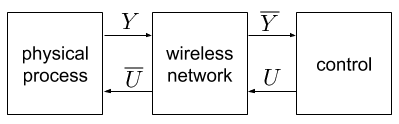
\includegraphics[width=0.95\columnwidth]{diagrams/fbd-system}
	\caption{Functional block diagram of a cyber-physical system in which a physical process and an automation system interact through a wireless network.}
	\label{fig:fbd-system}
\end{figure}

An alternative to schematic diagrams is SysML~\cite{SysML2017}. SysML is a general purpose modeling language that is often used for model-based systems engineering (MBSE) practice within industrial systems~\cite{MBSEandSysML}. SysML provides structural, behavioral, and parametric semantics for the analysis of complex systems. For examples, systems analysis using SysML enables capturing and communicating system requirements and design which include hardware, software, firmware, information flows, and processes with graphical notations. Within the factory automation industry, engineers are adopting SysML in the form of MBSE to develop realizable operational models of the factory and data flow processes. MBSE models address verification of design through executable simulations depending on the modeling tool.  The SysML specification is defined in~\cite{SysML2017}.  In SysML, the basic semantic constructs of the language are Packages, Blocks, Ports, Interfaces, and Constraints, in addition to the constructs provided by the Unified Modeling Language (UML). Packages are logical grouping of model elements. Package relationships are captured using the package diagram (PKG). Relationships of these constructs are captured in the block definition diagram (BDD).  The internal composition and connectivity of parts are captured in the internal block diagram (IBD). SysML includes other types of diagrams and semantic constructs that are not required for this analysis and are not explained here. The SysML model is comprehensive; however, the size and number of diagrams within the model are too extensive to include within this paper.  Therefore, the reader is encouraged to explore the SysML model defined in~\cite{SysML.Candell2018}.  A useful primer on SysML may be found in~\cite{Friedenthal2015.SysML}. 

Examples of the use cases and methodologies of using different graphical models for the analysis of manufacturing systems are explored in~\cite{Lutjen2015.GramosaMethod,Luder2011.GraphicalModeling,Jia2013.GraphicalModeling,Alvarez2013.GraphicalModeling}.  In~\cite{Quinsat2017.SysML}, SysML is used to capture both composition and behavior of an additive manufacturing work-cell.  A survey of applying graphical modeling languages in capturing information flows within a product service system which may be applied to manufacturing enterprises~\cite{Durugbo2011.GraphicalModeling}.  Our approach compliments these previous examples by combining the operational and wireless information transport systems together in a single model, thereby facilitating a single model that may be used for simulation and other systems engineering analyses.

While various architectures for the work-cell exist as exemplified in the literature, a common language and framework for communicating architecture and information flow has not been established for cross-domain interactions between the manufacturing system and its supporting communication networks.
SysML contains the semantics for such engineering capture and provides an industry accepted language for communicating composition, interfaces, and information flow. Moreover, SysML provides the semantics for assigning properties to any model element such that those properties are made  available for analysis using other tools such as Prot\'eg\'e \cite{StanfordUniversity.Protege} and the Web Ontology Language (OWL) \cite{W3C2012.OWL}.
It is important to understand that while SysML provides semantics for a formal capture of architecture, information flow, and parametric constraints, it may also be used for a higher-degree of abstraction provided by the functional block diagrams.  

\section{Conceptual Representation} \label{sec:conceptual}
The remainder of this work describes a reusable model for representing a comprehensive wireless factory work-cell using the semantic constructs of SysML.  We now follow with an exposition of our model beginning with the conceptual model followed by a detailed description of each component within the model. When discussing the model, the SysML term, \textit{block}, is omitted for the sake of brevity where the meaning is clear. 
\subsection{Packages}
The factory work-cell is decomposed into one general and nine major structural packages as shown in Fig.~\ref{fig:pdd-workcell}.  Packages include major logical groupings of structure within the model.  These packages are enumerated in the following paragraphs.

\begin{figure}[t]
	\begin{center}
		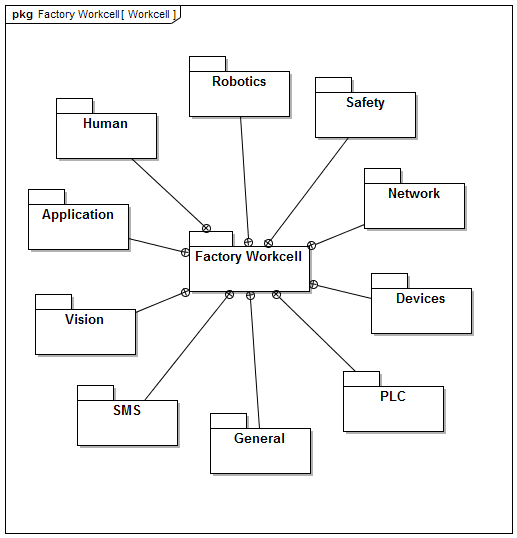
\includegraphics[width=0.95\columnwidth]{diagrams/pkg__Factory_Workcell__Workcell}%
		\caption{SysML package diagram showing the logical containment of the factory work-cell structural elements.}%
		\label{fig:pdd-workcell}
	\end{center}
\end{figure}


\subsubsection{General} A set of reusable structural elements that is used for conceptual modeling or extended to produce more complex model elements.  Each of the sub-packages within the General package extends basic features.  The sub-packages within General include time and constraints for data, electro-magnetics, and motion.

\subsubsection{Network} Describes the components, blocks, interfaces, and limiting factors of the industrial wireless network (IWN).  The IWN is modeled as the radio channel and the services provided by the network. Limiting factors are modeled as parametric equations associated with the radio channel and the services.

\subsubsection{Application}  This package contains the model elements describing a component of behavioral functionality typically implemented within software or firmware but could be implemented in hardware.  It describes the features and constraints of factory operation such as the logic of a supervisory controller or the feedback controller of a robot arm.  The Application sets the performance requirements of the wireless network, i.e., the factory network performance requirements are derived from the requirements of the applications deployed to a work-cell.

\subsubsection{Devices} Describes the types of devices found within the factory work-cell to include any device that interacts with the environment such as wired and wireless input-output (IO) devices including sensors and actuators.

\subsubsection{Robotics} Describes the computational and communicative components of robot control including sensing, actuation, and command.  Description of the robot itself is inconsequential to communication and therefore not included in the model.

\subsubsection{PLC} Describes the supervisory control components commonly handled by one or more programmable logic controller (PLC) components.  This package includes the elements responsible for coordination of actors and handling of most input-output.

\subsubsection{Safety} Describes the allocation of safety qualities typically included in the supervisory controller.  The Safety package includes devices, monitoring, and actuation of the safety behaviors within the factory work-cell.

\subsubsection{Vision} Describes the allocation of features to optical monitoring and tracking which are typical to the collaborative robotic work-cell.

\subsubsection{Spectrum Monitoring System (SMS)} Describes the qualities and interfaces of a factory spectrum monitoring system projected into the factory work-cell.  The SMS includes monitoring nodes and agents localized to the work-cell and connected to the automation system for real-time adaptation to changing multi-path and interference. 

\subsubsection{Human} Describes the features associated with human beings such as human motion, tasks, and carried equipment such as portable computing and communication devices.
\vspace{3mm} 

Several examples of how to use the model are provided within the model\cite{SysML.Candell2018}.  Examples include: a robotic force-torque leader-follower, a robotic force-torque limiter, a collision avoidance, and a robotic pick and place work-cell.  The parametric constraints are provided as examples and are intended to be used for communication to project stakeholders or replaced with executable computer code such as MATLAB or Python scripts, thereby making the model useful for simulation depending on the modeling tool selected.

\begin{figure*}
	\centering
	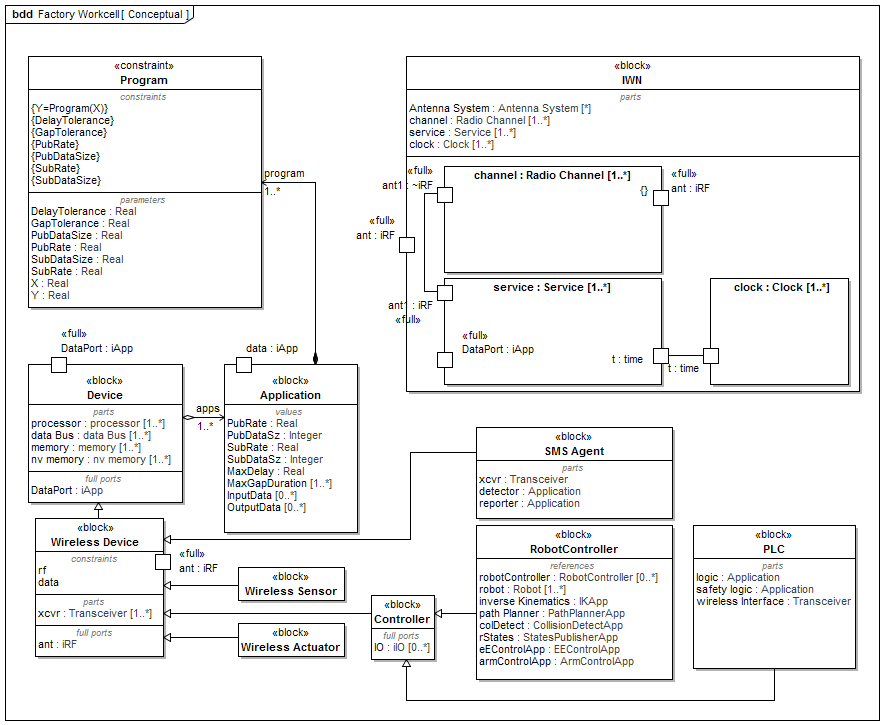
\includegraphics[width=0.97\textwidth]{diagrams/bdd__Factory_Workcell__Conceptual}%
	\caption{Architecture of the conceptual work-cell captured as a SysML block definition diagram.  In this diagram, only the most generalized blocks necessary to construct a work-cell scenario are shown.  More application-specific scenarios may be developed by deriving new blocks from the constructs shown here. The shapes and connectors used for expressing this model are defined in the SysML specification\cite{SysML2017}. }%
	\label{fig:conceptual:bdd}
\end{figure*}

\subsection{Conceptual Architecture}\label{sec:architecture}
The conceptual architecture of the wireless work-cell model is depicted in Fig.~\ref{fig:conceptual:bdd}. All the packages are included in this architecture, and the connections and relations between blocks are defined using the SysML semantics. This figure serves to orient the reader during the presentation of detailed model decomposition in Section~\ref{sec:detailed-model}. The work-cell model is composed of at least one Industrial Wireless Network (IWN) block and at least one Device block. More IWN blocks are used when multiple wireless networks coexist within the industrial work-cell. Applications are associated with Devices and performance constraints are applied to Applications. In this model, the Wireless Device is a subclass of Device, and the Controller is a further derivation of the wireless device. Moreover, the Controller is an abstract specialization of a wireless device that represents all types of devices intended to control other processes. The behaviour of a PLC or Robot is represented through two packages in the model. The production related behaviour is represented through the corresponding packages and the connectivity behaviour is represented through Devices such as the Robot Controller and the PLC which are special classes of Wireless Device containing all of the structure and behavior of the wireless device. Finally, an often overlooked component of any industrial wireless deployment is the spectrum monitoring system represented by the SMS Agent. Blocks in the model communicate through ports such as the \textit{ant} port which represents the antenna or waveguide interface.  Composition is further implied by the parts, constraints, and parameters associated with each block. These are listed within the compartments of each block.

\section{Detailed Model Decomposition}\label{sec:detailed-model}
In this section, we describe in detail the decomposition of the model packages. The decomposition of each package includes the properties and the components of the package where the relation between the package and physical industrial work-cells is illustrated. Moreover, some of the packages may have various types with different properties and hence sub-packages are defined for these packages. This section also includes a general explanation of the packages rules in the work-cell and the behavioral interactions between the packages.      

\subsection{General Package}
The General package contains the reusable elements of the model.  In particular, the General package contains elements that are not particular to any one work-cell component but can be reused or applied across several.  The concepts of time, clocks, and synchronization are included within General.  Moreover, several types of constraints are defined.  

\subsubsection{Time}
Time is an important construct within communication systems as well as industrial control systems.  Time is realized as a set of one or more clocks. A work-cell will contain one to several clocks typically embedded within each device to allow those devices to synchronize to a common clock. The local clocks within the work-cell devices will synchronize to a master reference clock and usually one with a high degree of precision, accuracy, and stability.  The degree to which the local clocks synchronize to the master will depend on the requirements of the applications that the local clocks serve.  Clock synchronization can be costly in power, size, and monetary cost of the devices, but it may be necessary depending on the applications using a clock.  Clock performance is a key driver of size and power consumption, and synchronization of clocks across a wireless network can be a challenge and is a highly studied field~\cite{ClockSync.Mahmood2017,ClockSync.Geetha2017}. Moreover, the Time package includes a constraint, Clock Performance, to represent the production of time and synchronization with a master clock. 

\subsubsection{Constraints}\label{sec:general:constraints}
Constraints provide limitations on the performance of an element within the model.  Within General, several constraints are defined which may be applied to any block within the model. These constraints include motion constraints, radio channel constraints, and networking constraints as shown in Fig.~\ref{fig:constraints:motion}-\ref{fig:constraints:network}.  

\paragraph{Motion Constraints}\label{sec:constraints:motion}

\begin{figure}[tbp]
	\centering
	\subfloat[Motion Constraints\label{fig:constraints:motion}]{%
		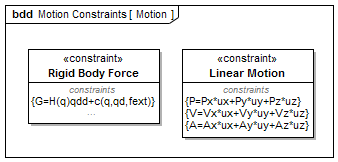
\includegraphics[width=0.95\columnwidth]{diagrams/bdd__Motion_Constraints__Motion}}
	\hfill
	\subfloat[Radio Channel Constraints\label{fig:constraints:radio}]{%
		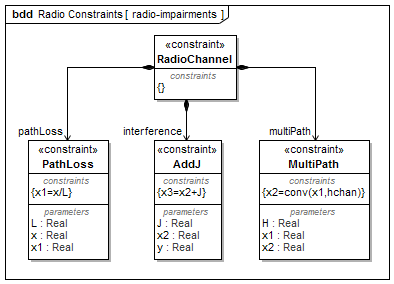
\includegraphics[width=0.95\columnwidth]{diagrams/bdd__Radio_Constraints__radio-impairments}}
	\hfill
	\subfloat[Networking Service Constraints\label{fig:constraints:network}]{%
		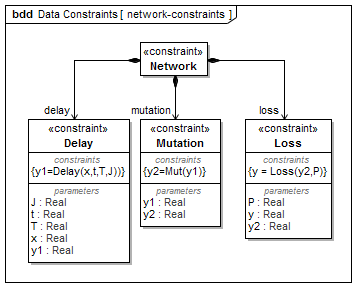
\includegraphics[width=0.95\columnwidth]{diagrams/bdd__Data_Constraints__network-constraints}
	}  
	\caption{Generalized network constraints consisting of rigid body motion~\protect\subref{fig:constraints:motion}, the radio channel~\protect\subref{fig:constraints:radio} and the network services~\protect\subref{fig:constraints:network}.}
	\label{fig:general:constraints}      
\end{figure}

When applied, these constraints provide the bounds of dynamical performance.  For example, motion constraints determine the positions, velocities, and accelerations on a rigid body.  The force vector equations \eqref{eq:robot:dynamics} are the general governing dynamic laws of motion as forces on a vector of joints as exerted by the end-effector or set of end-effectors on the environment.  The equations constrain the robot to operate according to the laws of physics, where the joint-space inertia matrix, $H$, is an ${n}\times{n}$ symmetric, positive-definite matrix, and $q$, $\dot{q}$, and $\ddot{q}$ are vectors of position, velocity, and acceleration, respectively.  The variable $f_{ext}$ is the six degrees of freedom (DOF) force acting on the end-effector, and $c$ is the joint-space bias force required to produce a zero sum force on the end-effector~\cite{Featherstone2007}.  
\begin{equation}
\label{eq:robot:dynamics}
\Gamma = H(q) \ddot{q} + c(q,\dot{q},f_{\!ext})
\end{equation}    
where $\Gamma$ is the vector of forces exerted by the end-effectors.  

This system of equations is controlled using a combination of digital feed-forward and feedback compensation in which the communication mechanism of the robot states directly impacts the controller's effectiveness. Joint control via a wireless network connection is typically avoided; however, monitoring of the linear and angular forces represented by $f_{\!ext}$ as sensed by a 6-DOF force-torque (FT) wireless sensor can be advantageous for many industrial applications.  As such, the performance of the wireless connection between a FT sensor and the controller can be a limiting factor in the performance of force-sensitive applications. Such a constraint may be applied to robot manipulators as defined in Section~\ref{sec:robotics}.

\paragraph{Radio Channel Constraint}\label{sec:constraints:radio}

The radio channel constraint limits wireless information flow to the laws of propagation which includes path loss, reflection, diffraction, and interference.  By applying this constraint to Wireless Devices described in Section~\ref{sec:devices:wireless-device}, such devices experience the effects of a lossy communication medium. The radio channel when applied to a wireless communication link within the work-cell manifests itself in accordance of the illustration of Fig.~\ref{fig:par:iwn-radio}.  The parametric equations for the radio channel include path loss, multi-path, and interference.  Path loss is generically modeled as the input signal divided by the bulk power loss in the channel. Path loss is often characterized as a two-piece linear function of distance\cite{Candell2017.NIST1951}. Multi-path is modeled as convolution of the transmitted radio signal with a linear time-varying impulse response characterizing the electromagnetic propagation between transmitter and receiver antenna systems.  Interference is then modeled as an additive component with power, bandwidth, and probability of excitation.

\begin{figure}[tbp]
	\centering
	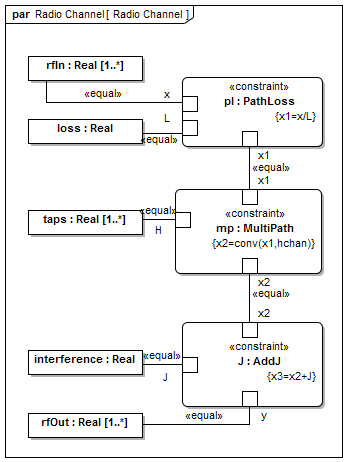
\includegraphics[width=0.95\columnwidth]{diagrams/par__Radio_Channel__Radio_Channel}%
	\caption{SysML parametric diagram of the radio channel constraints of the industrial wireless network.}%
	\label{fig:par:iwn-radio}
\end{figure} 

\paragraph{Data Constraints}\label{sec:constraints:data}

\begin{figure}[tbp]
	\centering
	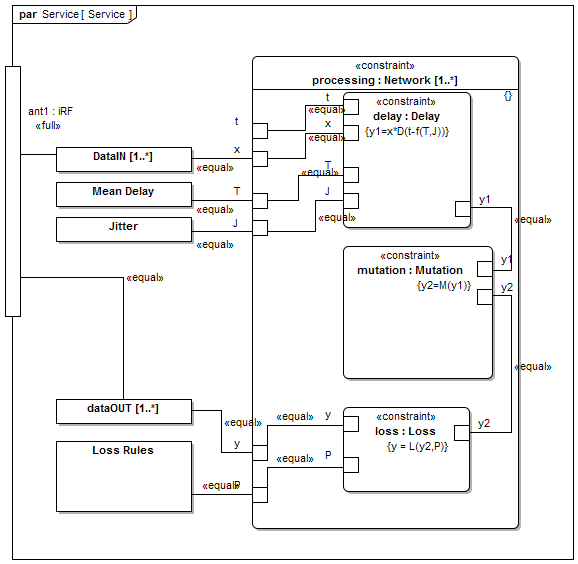
\includegraphics[width=0.95\columnwidth]{diagrams/par__Service__Service}%
	\caption{SysML parametric diagram of the data constraints applied to the industrial wireless network.}%
	\label{fig:par:iwn:data}
\end{figure}    

Delay, mutation, and loss of information within the industrial wireless network are encapsulated by the Network constraints block.  The Network constraint is applied to wireless devices within the network and represents the impacts of the radio channel and network components and protocols.  These constraints are illustrated in a parametric diagram of Fig.~\ref{fig:par:iwn:data} in which the rules for delay, mutation, and loss are applied to a service of an industrial wireless network within a work-cell. As with any constraint, the rules for data loss may be modeled as equations, psuedocode, or executable computer code such as MATLAB script or C.  These rules decide if information is lost due to delay or mutation.  While it is easy to understand how mutation leads to loss through a mechanism such as a checksum, unacceptable delay can also lead to loss of data.  

% equations for data constraints
Delay is simply a function of time, the physical environment of the factory work-cell, and state of the network at time, $t$. Many features of the network and the physical environment will have an impact on the output of the delay equation and will include data transmission duration, radio wave propagation delay, signal-to-noise, protocol for reliability, routing, internal queuing, and processing. A generalized equation for information delay by the wireless network is given as the sum of processing delay, queuing delay, transmission delay, and propagation delay. Subsequently, information loss is modeled as a set of rules governed by the attributes of the network infrastructure, transport medium, and protocols shown in~\eqref{eq:network-loss}. These rules may include thresholds for unacceptable delay and the ability of the network to correct for data mutation or loss in the physical channel (i.e. the air interface).

\begin{equation}\label{eq:network-loss}
\mathcal{Y}(t,\mathcal{X},\mathcal{N}) = 
\begin{cases} 
\mathcal{X} & \text{if } \mathcal{X} \vdash \mathcal{L}(t,\mathcal{X},\mathcal{N}) \\
\emptyset   & \text{otherwise}
\end{cases}
\end{equation}
where $\mathcal{X}$ and $\mathcal{Y}$ are blocks of data traversing the network and $\mathcal{N}$ is the state of the network at time, $t$.	We model the loss constraints as a general set of rules, $\mathcal{L}$, taking into account that each network system will have a different set of configuration attributes and protocols.  The rules will therefore change for each operational system and the networks used.  When the rules for loss are applied, the output of the network, $\mathcal{Y}$, becomes the input to the network, $\mathcal{X}$, when $\mathcal{X}$ satisfies $\mathcal{L}(t,\mathcal{X},\mathcal{N})$.

\subsection{Application}\label{sec:application}

\begin{figure}[tbp]
	\centering
	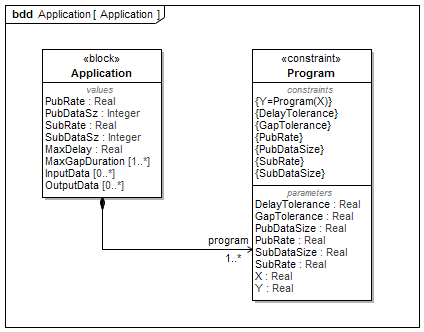
\includegraphics[width=0.95\columnwidth]{diagrams/bdd__Application__Application}
	\caption{Block definition diagram of the Application.}
	\label{fig:application:bdd}
\end{figure}

Applications, commonly implemented as software and firm-ware, represent the intelligence of devices. The application defines the behavior and the information flow requirements of the work-cell~\cite{appWorkcell1996, appWorkcell2001, appWorkcell2011}.  As defined in the model, without Applications implemented in software, firmware, or hardware, the work-cell devices would not function.  The definition of the Application block is shown in Fig.~\ref{fig:application:bdd}.  The Application block is constrained by the Program constraint which defines the logic of the program, its expected data flow input rates, and its tolerances to delay and information loss.  Devices host multiple applications each with a unique set of constraint properties.  It is essential when constructing a work-cell model that each application is identified and modeled appropriately.  An example of an Application is a collision detection system within a robot controller. Table~\ref{tab:sample:constraints} illustrates sample parameters used in the collision detector Application.

% 	\vbox{%
% 		\begin{description}[align=left, labelindent=5mm]
% 			\label{fig:CollDet:example}
% 			\item [Program] Collision Detector
% 			\item [Constraints] ~
% 			\begin{description}[align=left]
% 				\item[Input Data] robot states, 1 KB
% 				\item[Subscription Rate] robot states, 125 \si{\Hz}
% 				\item[Max Delay Tol.] robot states, 47 \si{\us}
% 				\item[Max Loss Duration] robot states, 275 \si{\ms}
% 			\end{description}
% 		\end{description}
% 	}

\begin{table}[tbp]
	\caption{Constraints Pertaining to a Collision Detector} \label{tab:sample:constraints}
	% Table generated by Excel2LaTeX from sheet 'constraints'
	\begin{tabular}{lc}
		
		\textbf{Constraint Property} &
		\textbf{Typical Value}
		\\
		\midrule
		Input Payload Size &
		1 KB
		\\
		Subscription rate &
		125 Hz
		\\
		Maximum Delay Tolerance &
		47 $\mu$s
		\\
		Maximum Loss Duration &
		275 ms
		\\
	\end{tabular}%
	
\end{table}

Specification of Application constraints provides a clear picture of the requirements of the factory automation system which can be projected on the wireless network. Through this process, it is possible to determine such requirements as scalability, throughput, reliability, and latency of the supporting network services modeled as radio and data constraints in Section~\ref{sec:general:constraints}. Indeed, as the manufacturing system becomes more complex and wireless becomes essential to communication, the projection of manufacturing requirements onto the wireless communication system becomes less clear.  Frequency planning, transmission scheduling, and error correction schemes become less obvious, and considerations of power, reliability, latency, and scale become optimization trade-offs. Such analyses are not within the scope of this paper but are important considerations for future research of manufacturing systems.  As such, the architectural elements and information flows exposed by an abstract model are a necessary first step.

\subsection{Industrial Wireless Network}

Central to the automation system is connectivity among devices and controllers~\cite{controlWSAN2010}.  More specifically, modern automation systems often employ networks to conduct inter-device communication~\cite{wirelessAutomation2017}.  The term \textit{inter-device} is appropriate as the Device block serves as the basis for all other components that communicate through the network.  Our model of the IWN is composed simply as a radio channel, a set of services, and a set of clocks as shown in Fig.~\ref{fig:iwn:bdd}.  This simplification of the model is necessary to allow the users of the model to provide as much or as little detail of the implementations of the radio channel and underlying services as required for their implementations.

\begin{figure}[tbp]
	\centering
	\subfloat[\label{fig:iwn:bdd}]{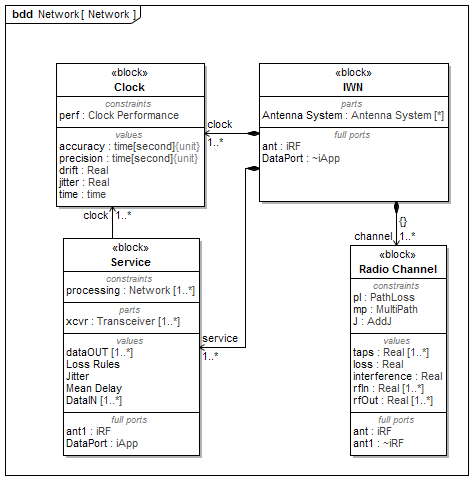
\includegraphics[width=0.99\columnwidth]{diagrams/bdd__Network__Network}}
	\hfill
	\subfloat[\label{fig:iwn:ibd}]
	{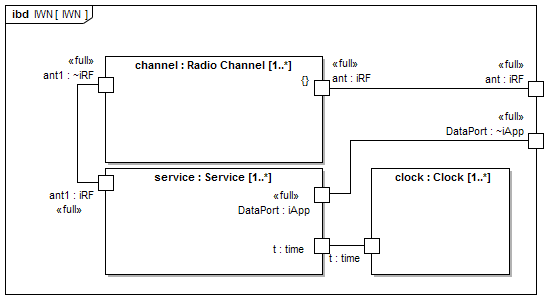
\includegraphics[width=0.99\columnwidth]{diagrams/ibd__IWN__IWN}}
	\hfill
	\subfloat[\label{fig:iwn-services:ibd}]
	{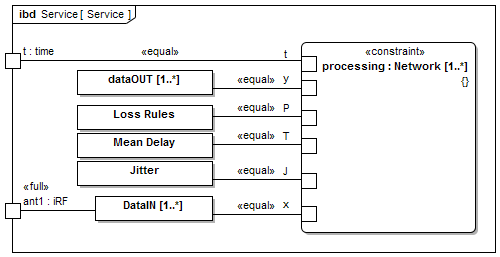
\includegraphics[width=0.99\columnwidth]{diagrams/ibd__Service__Service}}\\
	\caption{The BDD~\protect\subref{fig:iwn:bdd} and IBD~\protect\subref{fig:iwn:ibd} of the industrial wireless network with parametric IBD~\protect\subref{fig:iwn-services:ibd} of the Services block.}
	\label{fig:iwn:ibd:full}
\end{figure}

Connectivity of a constructed IWN is shown in Fig.~\ref{fig:iwn:ibd}.  An IWN is internally modeled such that information flows as radio frequency (RF) energy through the \textit{ant} port.  A radio channel is applied, theoretically for each pairwise link, and the modified signal is passed to the services for processing.  Network processing is modeled by the properties of network constraints as defined in Section~\ref{sec:constraints:data}.  Once processed by network services, information is routed back through the radio channel through the \textit{ant} port to other Devices connected to the IWN.  Moreover, the Service block includes a parametric model as shown in Fig.~\ref{fig:iwn:ibd:full}. This IBD with exposed parametrics exemplifies the inclusion parameters such as information delay and loss caused by the IWN, but it also exemplifies the impact of protocols and infrastructure (throughput, memory, etc.) within the network.  These effects are modeled as rules of loss shown in~\eqref{eq:network-loss}.

\subsection{Devices}\label{sec:devices}

\subsubsection{Device}\label{sec:devices:device}

A Device, defined in Fig.~\ref{fig:bdd:devices}, is generic construct representing an element within the work-cell with processing, memory, and storage capability. Devices have the capability to run applications as defined in Section~\ref{sec:application}.  Devices are sub-classed into Sensor and Actuator devices which generically refer to any type of sensor or actuator, and, in particular, the wired variety.  The Device is further sub-classed to the Wireless Device which is the central theme of our analysis.  Derived from the Wired Device are the Wireless Sensor and Wireless Actuator as well as the Controller.  The Controller represents the base class for deriving work-cell devices such as the PLC and the Robot Controller, sections~\ref{sec:plc} and~\ref{sec:robotics}, respectively, and provides support for external input-output (IO).

\begin{figure}[H]
	\centering
	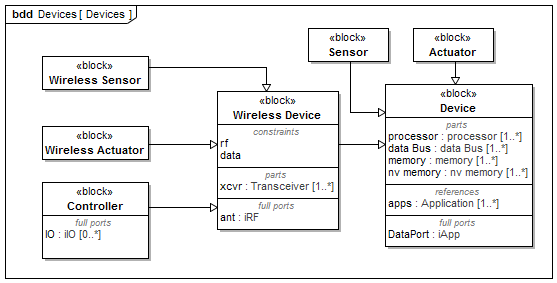
\includegraphics[width=0.95\columnwidth]{diagrams/bdd__Devices__Devices}%
	\caption{SysML block definition diagram of wireless devices within the factory work-cell.}%
	\label{fig:bdd:devices}
\end{figure}



\subsubsection{Wireless Devices}\label{sec:devices:wireless-device} 
A Wireless Device is a subclass of Device that contains the various components necessary for untethered communication.  These devices then communicate with each other through one or more industrial wireless networks (IWNs) which contains antenna systems, transceivers, protocols, and network services.  The relationships and composition of the Wireless Device are illustrated in Fig.~\ref{fig:wirelessdevice:full}. As shown, the wireless device is composed of at least one transceiver and each transceiver is composed of at least one antenna system which is composed of at least one antenna element.  The antenna system is constrained by its gain profile.

\begin{figure}[tbp]
	\centering
	\subfloat[Block definition diagram of the Wireless Device\label{fig:wirelessdevice:bdd}]{%
		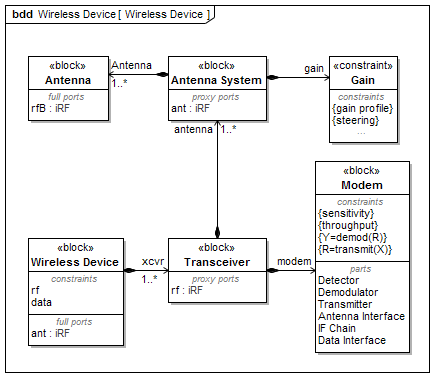
\includegraphics[width=0.95\columnwidth]{diagrams/bdd__Wireless_Device__Wireless_Device}
	}
	\hfill
	\subfloat[Internal block diagram of the Wireless Device\label{fig:wirelessdevice:ibd}]{%
		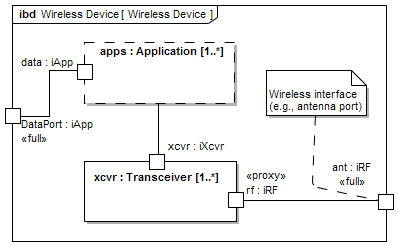
\includegraphics[width=0.95\columnwidth]{diagrams/ibd__Wireless_Device__Wireless_Device}
	}  
	\caption{Block definition diagram~\protect\subref{fig:wirelessdevice:bdd} and the internal block diagram~\protect\subref{fig:wirelessdevice:ibd} of Wireless Device.}
	\label{fig:wirelessdevice:full}      
\end{figure}

\subsubsection{Test Device}\label{sec:test-device}

\begin{figure}[tbp]
	\centering
	\subfloat[Block definition diagram of the Test Device\label{fig:testdevice:bdd}]{%
		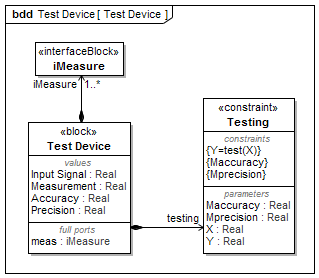
\includegraphics[width=0.95\columnwidth]{diagrams/bdd__Test_Device__Test_Device}
	}
	\hfill
	\subfloat[Internal block diagram of the Test Device\label{fig:testdevice:ibd}]{%
		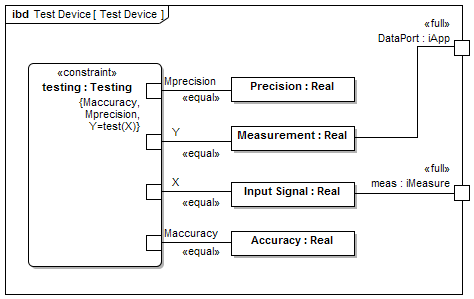
\includegraphics[width=0.95\columnwidth]{diagrams/ibd__Test_Device__Test_Device}
	}  
	\caption{Block definition diagram~\protect\subref{fig:testdevice:bdd} and the internal block diagram~\protect\subref{fig:testdevice:ibd} of Test Device.}
	\label{fig:testdevice:full}      
\end{figure}

The Test Device is a subclass of Device that represents devices used for calibration or ground truth testing of properties of a work-cell.  The block definition and internal configuration are illustrated in Fig.~\ref{fig:testdevice:full}.  A Test Device is constrained by its accuracy and precision as well as the algorithm for controlling measurement.  An example of a test device is a calibrated force sensor that may be used as comparison to a 6-DOF wireless sensor mounted on the wrist of a robot arm as shown in the top left of Fig.~\ref{fig:workcell:examples}. Test devices are useful and necessary elements of the wireless testbed to establish accurate and repeatable ground truth measurements.  For example, a stationary precision force sensor may be used to establish a ground truth force value, and a high-accuracy vision tracking system is used for truth in position.  Test devices are modeled such that measurements may traverse the operational wireless network or a stand-alone wired interface.

\subsection{Robotics}\label{sec:robotics}
\begin{figure}[tbp]
	\centering
	\subfloat[Block definition diagram of the Robot Controller\label{fig:robotcontroller:bdd}]{%
		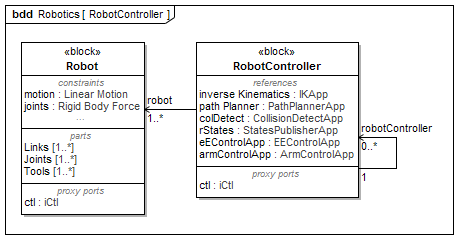
\includegraphics[width=0.95\columnwidth]{diagrams/bdd__Robotics__RobotController}
	}
	\hfill
	\subfloat[Internal block diagram of the Robot Controller\label{fig:robotcontroller:ibd}]{%
		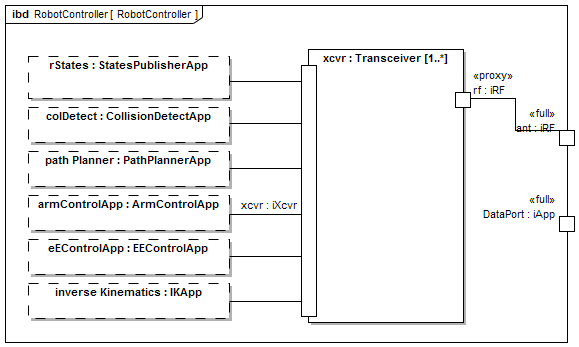
\includegraphics[width=0.95\columnwidth]{diagrams/ibd__RobotController__RobotController}
	}  
	\caption{The BDD~\protect\subref{fig:robotcontroller:bdd}, IBD~\protect\subref{fig:robotcontroller:ibd} of the Robot Controller.}
	\label{fig:robotocontroller:full}	
\end{figure}

The robotics package contains elements specific to robot systems.  Robot systems are composed of at least one robot controller associated with one or more robots, as shown in Fig.~\ref{fig:robotcontroller:bdd}.  In manufacturing, robots interact with their surrounding to accomplish assigned tasks such as tending machinery, moving materials, welding, and inspecting. Robot controllers provide support for external IO devices.  In addition, modern robot controllers will support a variety of open and proprietary network protocols allowing for interaction with other actors in the work-cell.  The robot controller's main task is control of the rigid body dynamics of the robots which is usually conducted via real-time communication over a high-throughput serial field-bus. While joint control is conducted using wires, the robot controller is responsible for other tasks requiring reliable, low-latency communication in which wireless may serve a role.  These tasks are captured in the model as applications (Fig.~\ref{fig:robotcontroller:ibd}) and explained as follows.

\begin{description}
	
	\item[\textbf{Robot States Publisher}] Transmission of robot states to external actors such as other robot controllers, supervisors, and safety systems.
	
	\item[\textbf{Arm Controller}] Also known as manipulator control, serves to accept position commands as Cartesian or joint space trajectories and waypoints from other actors within the work-cell.
	
	\item[\textbf{End Effector Control}] Command and control of the robot end-effector such as a gripper or sensor.  The end-effector may be equipped with a high-throughput wireless sensor necessitating reliable communication.
	
	\item[\textbf{Inverse Kinematics}] Converts Cartesian coordinates of the end-effector into joint positions.
	
	\item[\textbf{Path Planner}] Determines the optimal geometrical trajectory to achieve a final pose given knowledge of self-collision and real-time knowledge of the surround environment.  Path planning is a sophisticated part of a robot system and may be allocated to an external system depending on throughput and latency requirements.
	
	\item[\textbf{Collision Detector}] This application monitors the states of other actors and obstructions within the work-cell. If possibility of collision is detected, the collision detector takes action.
	
\end{description} 

These applications within the robotic work-cell define many information flows requiring careful analysis to achieve reliability and latency necessary for the safety and control of the manufacturing process. Information flows are identified in Section~\ref{sec:wireless-infoflows}.

\subsection{PLC}\label{sec:plc}
The PLC is a specialized class of Controller.  PLCs were originally developed to mirror relay circuits in software; however, the modern PLC is much more advanced and is usually equipped with multiple processors, a real-time operating system (OS), and capabilities to support various types of industrial IO devices.  In addition, modern PLCs (also called automation servers) include both a general purpose OS with a real-time kernel and multiple network interfaces.  Many network-routable protocols are also supported.  With the addition of wireless protocols, PLCs now have the ability to support IO devices connected remotely without wires.  Supervision of untethered robots is also possible using PLCs.  The PLC is modeled as a Controller device with the work-cell model.  Shown in Fig.~\ref{fig:PLC:ibd}, the PLC is modeled as a wireless device with transceiver, logic application, and safety applications.  More sophisticated PLCs may be modeled by extending the PLC block.  As applications, the logic and safety functions are constrained by application constraints. Finally, as Controller devices, PLCs are modeled with an IO port, thus IO can be connected to the PLC by wires or by wireless network connection.

\begin{figure}
	\centering
	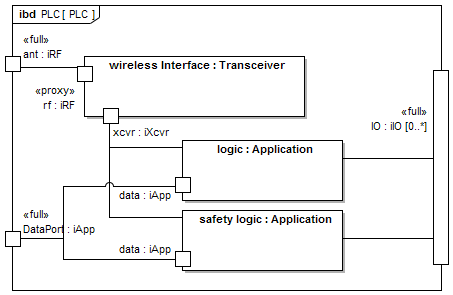
\includegraphics[width=0.95\columnwidth]{diagrams/ibd__PLC__PLC}
	\caption{The IBD of the PLC showing composition and connectivity of the control logic and safety logic Application instantiations to the Transceiver interface. }
	\label{fig:PLC:ibd}
\end{figure}

\subsection{Safety}\label{sec:safety}
% 	\textcolor{red}{MOHAMED TO WRITE}
% 	\textcolor{blue}{Allocation of safety features from the PLC. High availability IO input devices, output relays, used for E-STOP usually to protect life and property; constrained by response time requirement of the safety rating}

In a work-cell with interacting humans and robots, functional safety requirements are typically strict by specifying the rules related to four main safety criteria, namely, monitored stops, controlled speeds, separation distances, and power and force limits in order to prevent injury for humans and damage for equipment. The wireless safety package is composed of a safety controller and safety devices. Traditionally, the safety requirements of the work-cell is fixed and managed by the safety controller which receives safety-related measurements and takes the corresponding actions. Alternatively, the safety controller may be connected to the PLC where the current work-cell activities are supervised.  The PLC will determine the required safety rating and the safety controller behaves accordingly. The dedicated safety controller is needed to achieve the required high reliability and low latency safety requirements and it can be a general PLC with safety modules. 

The safety devices include non-safety-rated devices such as the various work-cell sensors and actuators and safety-rated input and output devices. Safety control input devices include Emergency-stop and enabling buttons while output devices include relays and switches for various work-cell equipment. The use of wireless in safety control loops allows installing a larger number of sensing devices including vision systems to monitor the human and robots activities, velocity and proximity sensors, and machine status sensors. Moreover, wireless allows to have mobile control panels where workers can activate a safety device at any time and location within the work-cell.        

\subsection{Vision}\label{sec:vision}
% 	\textcolor{red}{MOHAMED TO WRITE}
% 	\textcolor{blue}{composition (vision processing, optical devices with networking interfaces, general panning and zooming, object detection, interface to robotic system, interface to the supervisory system)}

%     \textcolor{green}{Make that we allow the following in your definition: part tracking, object detection, intput to collision avoidance systems, tracking of mobile robots, augmented reality devices/systems, security cameras, etc.}
The vision system considered in this subsection is the one used for work-cell monitoring and general object detection. It does not cover the machine-embedded vision systems which can be used for inspection and characterization of objects such as the shape, color, texture, or size of processed materials. The data collected by the work-cell vision system can be used for parts and mobile robots tracking, collision avoidance, object detection, security identification systems, and augmented reality devices and systems. The vision system communicates with the supervisory control, robotic controller, and the safety system to provide the work-cell state which contains the positions of various equipment, robots, and humans. 

The vision system is composed of optical devices, vision processing unit, and interfaces to various work-cell systems. The optical devices are the cameras for capturing images at high enough speed to track and detect various objects. These cameras have wireless network interfaces to be connected to the vision processing unit to allow collaborative processing of the captured images and obtaining precise work-cell state. The vision processing unit performs data acquisition from the distributed optical devices and feature extraction to detect and track the positions of various entities in the work-cell. 

The vision system communicates the corresponding data to the supervisory control, robotic control, and the safety system for decision making based on the captured work-cell state. The supervisory controller uses vision system data for robots and workers localization, parts detection and identification, and schedules tasks using this information. The robotics controller uses these data for motion control, path planning, and collision detection. Finally, the safety controller uses these data for safety requirements implementation such as enforcing safety stops, controlling the speeds of moving objects, and limiting power and forces of various work-cell components.    

\subsection{Spectrum Monitoring System}\label{sec:sms}
A spectrum monitoring system (SMS) is an often overlooked yet valuable part of the wireless factory work-cell with requirements specified in~\cite{Candell2017.SMS}.  The SMS is modeled as an atomic agent within the work-cell.  The SMS Agent is one component in a larger enterprise-level spectrum monitoring deployment.  The SMS agent shown in Fig.~\ref{fig:sms:bdd} includes a transceiver, an event detector, and a reporting agent.  The transceiver can be implemented as an RF-to-baseband converter.  The detector application is responsible for detection and estimation of anomalous spectral events and may employ machine learning to accurately detect anomalies and report localized spectral events.

The reporter application collects, filters, and reports event information to a central management console.  SMS reports support identification of long-term patterns such as growth trends in particular wireless bands.  Since the SMS Agent is part of a larger network of spectrum monitoring, it is presumed that reports are wirelessly transmitted back to the enterprise management console.  These reporting events use bandwidth otherwise used for the factory operation, thus reports must be made concise and infrequent.  This implies substantial filtering and intelligence in the local SMS agents This may provide opportunities for research.

Detection events may be routed to the local supervisor, robot controller, and safety system.  By leveraging spectral awareness, work-cells can be made safer and more reliable.  As SMS are not yet widespread in industrial applications; thus, standardized protocols are needed for reporting and integration with automation systems.

\begin{figure}[tbp]
	\centering
	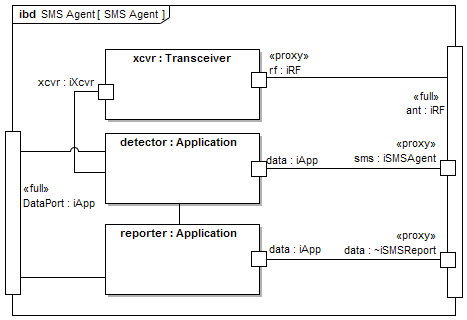
\includegraphics[width=0.99\columnwidth]{diagrams/ibd__SMS_Agent__SMS_Agent}
	\caption{Spectrum monitoring agent composed of transceiver, detection application, and reporting application.}
	\label{fig:sms:bdd}
\end{figure}

\subsection{Human}\label{sec:human}
% 	\textcolor{red}{Mohamed to write}
% 	\textcolor{blue}{People; wearable devices such as gas sensors, identification, and localization; could be security related for access control; portable devices; personal devices; include motion on factory floor; operational tasks; intervention of process      
% 		Composition, constraints of motion}

Humans can exist in a modern work-cell for short or long periods of time depending on the required task. Two categories of human-related aspects are captured in the work-cell model. First, the human existence in the work-cell leads to detection and identification of the corresponding worker for both safety and security. Also, human motion within the work-cell requires position tracking for environment monitoring and spectrum monitoring due to radio frequency channel variations with human movements. The second category includes the human interfaces with the work-cell process that include portable control devices, wearable sensors, and workers communication devices to get task commands. Moreover, depending on the process constraint, personal devices of workers may interfere with the work-cell communications if allowed.      

\section{Results of a Work-cell Case Study}\label{sec:wireless-infoflows}
% Rick's section	
\begin{figure*}[tbp]
	\centering
	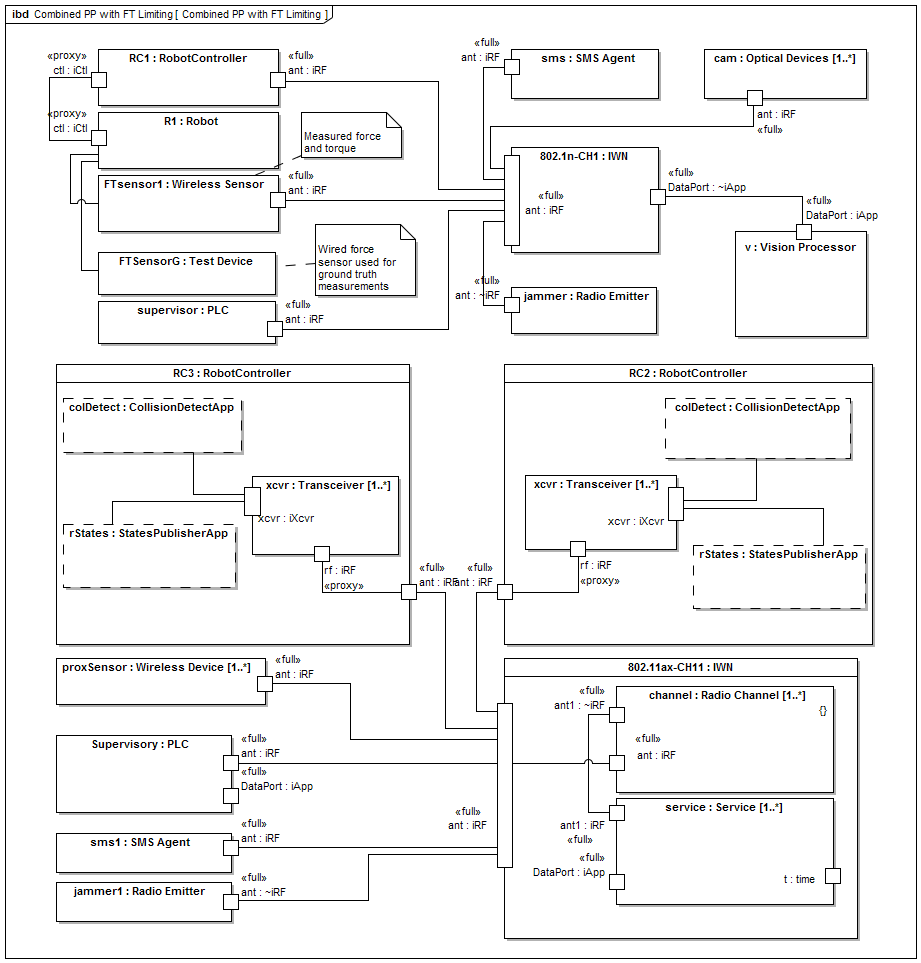
\includegraphics[width=1.05\textwidth]{diagrams/ibd__Combined_PP_with_FT_Limiting__Combined_PP_with_FT_Limiting}
	\caption{IBD of a work-cell employing multiple networks in collaborative robot operation coexisting with robot force limiting inspection station.}
	\label{fig:workcell:examples}     
\end{figure*}

In this section we present a case study of a work-cell which includes a force-torque limiter robot application and a two-robot collaborative pick and place operation.  The model for this system is depicted in Fig.~\ref{fig:workcell:examples}.  The number and type of wireless information flows will depend on the configuration of the work, the number of applications, and the places where wireless is applied. For this case study, the force limiter section is composed of a robot controller, a robot, and an FT sensor. A PLC is used for work-cell supervision, and a test device is deployed for ground truth measurement.  An SMS agent monitors the electromagnetic spectrum.  A Radio Emitter is included to model the transmission of interference.  An IEEE 802.11n network is represented in the model by an IWN block. Properties of the radio channel and services of the communication system are therefore represented. Similarly, another example is implemented in \cite{SysML.Candell2018} for a pick-and-place scenario where the model is composed of two robots, a PLC, an IWN, and an SMS Agent in addition to proximity sensors and an IEEE 802.11ax network.

Referring to these examples, typical information flows are easily identified as connections between Wireless Device blocks and the antenna port, \textit{ant}, of the IWN.  Recall that the IWN includes radio channel and services offered by the network itself.  Therefore, all wireless information flows will traverse the IWN through the \textit{ant} port.  Applications are implied and produce and consume the information according to associated constraint properties.  Information flows are generated by the interactions between actors and include the following:  

\begin{description}
	
	\item[\textbf{Robot States}] The geometry states of the robot such as position, velocity, and acceleration of each joint or end-effector. Robot states may include Cartesian or joint space readings depending on the need of other applications or the capabilities of publisher.  Robot states are usually transmitted at 30 Hz or faster~\cite{JMarvel2017}.
	
	\item[\textbf{Force Sensor Readings}] The readings from a sensor mounted on the wrist of each robot arm. These readings are typically in the format of wrenches (linear and angular forces) and are transmitted at rates from 15 Hz for monitoring applications up to 500 Hz for force limiting and control applications~\cite{onrobot}. Other sensors may produce data in the system such as proximity sensors which can generate data in the range of 1-50 Hz~\cite{DiffuseSensorSpecs} and Tactile sensors which can have information flow rates faster than 1000 Hz~\cite{TactileInternet}.
	
	\item[\textbf{Machine Health Monitoring}] Readings from sensors mounted within machinery such as mills, routers, and lathes used to sense and predict deviations of mechanical components from design tolerances. Readings for prognostics and health monitoring are often aggregated at the source with statistical metrics being communicated to a factory enterprise application; however, non-aggregated readings may also be transmitted to a remote signal analyzer.  Health monitoring sensors measure temperature, vibration, acceleration, inclination, position, and rates of change of angles. Information flows from a single aggregation point may reach 200 kB/s on average for a 6-DOF sensor apparatus described in~\cite{ELWeiss}. While the outputs of health monitoring sensors are usually wired into a local aggregation devices, it is desirable to transmit these readings to an on-line optimizer or PLC within the work-cell~\cite{Weiss2016.PHM}.
	
	\item[\textbf{IO States and Supervisory Messages}] These contain both the boolean-valued readings and commands from sensors, and task orders in the form of short commands and lists of instructions which can originate from any supervisor within the network such as a PLC or other controller. Sensor readings (inputs) and actuation commands (outputs) are transmitted in periodically or pseudo-randomly at rates indicative of movements of machinery and materials through the manufacturing process.  Typical analog and boolean IO states range from to 10 Hz to 100 Hz depending on the manufacturing process~\cite{TwinCAT}.
	% 		\item[Supervisory Messages] Directives and task orders in the form of short commands and lists of instructions and can originate from any supervisor within the network such as a PLC or other controller. Supervisory messages include state information such as task status from collaborating actors within the work-cell. 
	
	\item[\textbf{SMS Events}] The SMS agent will communicate state information and directives to controllers within the work-cell.  These messages allow the automation system to react under anomalous spectrum conditions within the work-cell. These information flows may be necessary for safe operation of the work-cell. The data rate of reports from an SMS agent without processing or compression can be in the range of 1 to 10 megabits per second (Mbps)~\cite{cuevas_2015}.
	
	\item[\textbf{Vision Applications}] The vision system will communicate videos or images for processing and decision making. Typical Video flows can have the rates of 30 Hz for surveillance and 125 Hz for motion capturing~\cite{industrialCCTV, ELWeiss}. Information flow for Object tracking systems can have the rate of 10-200 Hz depending on the tracked objects and the required accuracy~\cite{lidar, motioncapture}. 
\end{description}
%\vspace{5mm}


%     % THIS TABLE TO BE REMOVED 8/2/2018
% 	\begin{table}[tbp]
% 		\centering
% 		\caption{Work-cell information flows.}
% 		\label{tab:infoflows}
% 		\begin{threeparttable}
% 			%begin tabular
% 			% Table generated by Excel2LaTeX from sheet 'infoflows (2)'
\begin{tabular}{lccc}
\textbf{Information Flow} &
  \textbf{Information Rate (Hz)} &
  \textbf{Protocol} &
  \textbf{Citation}
  \\
\midrule
\textbf{Robotics} &
   &
    &
  
  \\
Joint states &
  30-1000 &
  Datagram &
  \cite{JMarvel2017}
  \\
Task states &
  1-5 &
  Reliable &
  TBS
  \\
End-effector commands &
  \tnote{*} &
  Reliable &
  TBS
  \\
Collision events &
  \tnote{*} &
  Reliable &
  TBS
  \\
\midrule
\textbf{Sensors} &
   &
    &
  
  \\
Force/Torque &
  15-500 &
  Datagram &
  TBS
  \\
Proximity &
  1-50 &
  Reliable &
  \cite{DiffuseSensorSpecs}
  \\
Tactile &
  $>$1000 &
  Reliable &
  \cite{TactileInternet}
  \\
\midrule
\textbf{Vision} &
   &
    &
  
  \\
Video &
  30 (Surveillance)-175 (motion capture) &
  Datagram &
  \cite{industrialCCTV, labOpticalCameraSpecs}
  \\
Tracking &
  10-100 &
  Datagram &
  \cite{LIDA15Hz}
  \\
\midrule
\textbf{Supervision} &
   &
   &
  
  \\
Command/control &
  1-5 &
  Reliable &
  TBS
  \\
IO States &
  10-100 &
  Reliable &
  \cite{TwinCAT}
  \\
\midrule
\textbf{Spectrum Monitoring} &
   &
   &
  
  \\
SMS Events &
  \tnote{*} &
  Reliable &
  TBS
  \\
SMS Reports &
  <1 &
  Reliable &
  TBS
  \\
\bottomrule
\end{tabular}%
%end tabular
% 			\begin{tablenotes}
%             	\item[] \textcolor{blue}{add information about the purpose of this table. What are the flow items, impact to bandwidth, and }
% 				\item[*] Indeterminate flow rate
% 				\item[] \textcolor{red}{need validation and citations}
% 			\end{tablenotes}
% 		\end{threeparttable}
% 	\end{table}

\section{Discussion and Conclusions}\label{sec:conclusion}
A model was developed using SysML. The developed model is constructed of the elements necessary to construct useful representations of factory work-cells in which wireless networks are used to transport information necessary for automated control system operation.  Reusable, derivable elements are developed and then extended to represent the constructs of the work-cell such as robot control, supervisory control, vision, safety, and spectrum monitoring.  An industrial wireless network is then developed and constraints of the radio channel and network services are formalized. Using the architectural model, information flows are explored and incorporated within. 

It is important to mention that this model includes an often overlooked component of any industrial wireless deployment which is the spectrum monitoring system and also considers the human-robot and robot-robot interactions in industrial environments. The current model includes various systems constraints including motion constraints, radio channel constraints, and networking constraints. The parametric constraints are provided as examples and can be replaced with executable computer code thereby making the model useful for simulation depending on the modeling tool selected. Furthermore, the applications within the robotic work-cell define many information flows requiring careful analysis to achieve reliability and latency necessary for the safety and control of the manufacturing process.

With increased dependency on wireless communications for more complex manufacturing systems, the projection of manufacturing requirements onto the wireless communication system becomes less obvious. Such analysis of this projection is essential for future research of manufacturing systems. As such, the architectural elements and information flows exposed by an abstract model
are a necessary first step. Our model in its current state of development is comprehensive enough to support architectural and ontological analyses of the factory work-cell.  As such, information about the relationships between components of a work-cell and attributes related to the wireless network may be discovered. Therefore, our model serves as a foundation for future systems engineering analyses. Moreover, our model may be used as a tool for academic and industry exploration of wireless testbed development.  We make the model openly available through GitHub at~\cite{SysML.Candell2018}.


\section{Introduction} \label{sec:intro}    
The fourth industrial revolution promises unparalleled productivity and capability advances in manufacturing. To support the manufacturing industry in this conversion, various programs have been established in several countries such as Smart Manufacturing in the U.S.~\cite{SmartManuf} and Industry 4.0 in Europe~\cite{Industry40, cpsInd4.0}. Propelled by economic pressure toward greater efficiency, factory agility, and product customization, future factories will have the technological ability to adapt to customer demands quickly, modify manufacturing processes automatically based on quality feedback, and fabricate products with a reduced environmental impact.  Technological advances required for smart manufacturing to be successful include collaborative and mobile robotics~\cite{indRobot2017}, distributed machine autonomy based on artificial intelligence \cite{ManufAI2009}, improved process observability~\cite{IIoToverview2018}, and a high degree of interconnectivity among automation resources~\cite{ieMag2018}. Work-cells are self-contained units of operation within a factory~\cite{CHEN2001199, JMarvel2017, 6059204}.  These work-cells are composed of various machines, conveyors, motors, edge devices, and robots.  Robots will work together and with people to accomplish complex tasks or to tending to other machines within the work-cell.  Robots will have the ability to roam between work-cells within a factory, learn their roles quickly, become aware of edge devices, and communicate with other actors within the work-cell to accomplish their goals. Efficient communications between robots and the other players in the work-cell are essential to the fulfillment of the robot-related tasks.

Current manufacturing architectures use wired connections through field-bus and industrial Ethernet protocols for sensing and real-time control~\cite{etherCAT, indPrinter}.  Indeed, through advances in time-sensitive networking, many of the promises of smart manufacturing are being realized; however, the true goals of smart manufacturing require a large deployment of sensing and actuation devices and mobile, perhaps autonomous, robotics actors~\cite{ieMag2018}.  The use of wires precludes mobility and makes deployment of edge devices more expensive as each  requires power, cables, and conduit for communication. By adopting wireless for both sensing and control of machines within the work-cell, a lower-cost, untethered operation is achievable\footnote{The power for untethered operation can be achieved through the use of rechargeable batteries to power the untethered machine or robot for enough operating period.}. Once wireless is adopted as the primary mode of communication, questions arise as to the required latency, reliability, and scale of the wireless network especially when the network is used for the control of machines and the assurance of safety~\cite{ieMag2018}. 

The work presented here addresses the present need for a comprehensive architectural model of the factory work-cell in which wireless is a preferred mechanism for carrying information within the work-cell. We begin with an architectural analysis of the future collaborative work-cell that includes edge devices, robots, vision systems, and supervisory controllers. Our architectural analysis includes structural components, information flows, and parametric elements of the work-cell. We identify factors that limit reliability, latency, and scalability of the wireless network, and we conclude with a discussion of significant information flows. Significant information flows are defined as operationally critical or safety-related.  Our contributions are:

\begin{itemize}
	\item[$\star$] First, we develop a comprehensive and extensible architectural model using the Systems Modeling Language (SysML) that provides primitives for describing the physical and networking components of a work-cell with parametric constraints\footnote{We make the model publicly available for download. A valid license of MagicDraw 18.5 is required to use the model.  A web-based report of the model is provided for read-only access.};
	\item[$\star$] Second, we provide a framework for analyzing cross-domain interactions of complex wireless work-cell deployments; and
	\item[$\star$] Third, significant information flows are identified, annotated with rate constraints.
\end{itemize}

The remainder of this paper is organized as follows:  In Section~\ref{sec:related-work}, previous related work is discussed and our motivation for constructing a model is presented.  A brief introduction to systems modeling is presented in Section~\ref{sec:systemsmodeling} and provides a primer on the SysML language. The conceptual architecture of the model providing a concept-of-usage is proposed in Section~\ref{sec:conceptual}, followed by a detailed exposition of each package in Section~\ref{sec:detailed-model}.  Then, in Section~\ref{sec:wireless-infoflows}, significant information flows are discussed through introducing a case study. Section~\ref{sec:conclusion} concludes the paper and identifies opportunities for future research.

\section{Related Work}\label{sec:related-work}

Current modeling work on factory work-cells is mainly aimed at defining and characterizing the subsystems, such as human staff, robots, and machine tools, in individual applications. By following blueprints (schematics) of production tasks, the work flow can be divided into separate assignments which are distributed by a task dispatch system to individual machines~\cite{IkeaBot}. Analytical models are thus obtained for performance analysis in work-cells. As an example, a mathematical model for real-time performance analysis of a gantry work-cell with robots is established with the timing and the randomness of tasks and disruptions are captured  \cite{8098604}. In \cite{OU2017212}, the same model is used to investigate the system natural properties such the system cycle and waiting times and to identify bottlenecks through studying the sensitivity of each machine. Similarly, the steady state analysis for production lines with uncertainties is performed through various decomposition methods~\cite{Colledani2013,doi:10.1080/00207543.2012.713137,doi:10.1080/00207540500385980}. In \cite{Colledani2013}, a decomposition method is presented for the analysis of continuous flow lines. The presented model is used to analyze flow lines with single and multiple failure mode machines and machines subject to aging and having up and down times. In \cite{doi:10.1080/00207543.2012.713137}, a model to evaluate the performance of transfer lines with unreliable machines and finite transfer-delay buffers is presented. A decomposition method is introduced to model the transfer line, using the general-exponential distributions instead of the exponential distributions to approximate the repair time distributions of the fictitious machines. In \cite{doi:10.1080/00207540500385980}, the authors present a model for evaluating the production rate and distribution of inventory of a closed-loop manufacturing system with unreliable machines and finite buffers. The model accounts for the different sets of machines that could cause blockage or starvation to other machines. In \cite{QChang,Liu2012}, the performance analysis modeling for serial production lines with disruptions is explored by studying the impact of each individual downtime event in terms of permanent production loss and financial cost. These analytical models generally work well for simple systems with small number of components or few interactions between various equipment. Also, the analytical models can be used to abstract industrial systems to understand various performance trends without studying various details. As a result, we introduce a comprehensive model that include network and production impacts on the industrial work-cell.  

Furthermore, the reconfigurable work-cell architecture is widely considered for automated manufacturing. The main advantage of reconfigurable work-cells lies in the flexibility of reconfiguration of work-cell components to adapt to varying production requirements where the assembly of the work cell is optimized for each specific task~\cite{CHEN2001199}. In the work-cell that hosts robots, robots are installed therein to allow for autonomous configuration within their workspace \cite{8023523,10.1007/978-3-319-65151-4_10,6059204}. Approaches and performance criteria for reconfigurable robotic systems have recent developments in control architectures to achieve various levels of reconfigurability \cite{Fulea}. The National Institute of Standards and Technology (NIST) has defined a Network of Things (NoT) model which can depict the structure of work-cells by a group of NoT building blocks and model the behaviors of individual components in a work-cell~\cite{NIST800-183}.  The NIST NoT model is focused primarily on sensor networks and the collection of data.  Actuation is cursorily noted, and, as such, cross-domain interactions between the physical system and the network are not addressed. Several other robotic work-cell architectures are discussed in the literature. In \cite{OpenArch}, a reference model for a control system functional architecture applied to open architecture robot controllers is presented. In \cite{CARPANZANO2007435}, a methodology to develop self-adaptive factory automation solutions is illustrated, using a novel modular simulation based method. With the increase in complexity and reconfigurability of work-cells, studying various production criteria and networks impacts requires introducing new models to capture these interactions and to be abstract enough to model different configurations and scenarios of industrial work-cells.  

In a work-cell model, data flows are used to capture the trajectory of system information exchange between work-cell components and identify their roles in specific operations~\cite{OpenArch}. For example, safety-related operations employ the vision system and various proximity sensors that generate proximity data and transmit them to the safety manager to define safety zones in an automotive assembly work-cell~\cite{safeeye}. 
In another example, data flows are enabled in a work-cell to capture human operator gestures from embedded cameras in human-robot collaborations~\cite{cobotcell}. These gestures can be later regenerated in simulators based on the transmitted position data from the field to optimize work-cell safety operations~\cite{gesture}. Currently, most of the work-cell information in these scenarios are transmitted by wired networks. Wireless networks have gained increasing interests to enable data flows in the highly connected work-cells. Wireless standard bodies have proposed their network reference models in factory environments which include the work-cell cases in the data-centric architecture~\cite{ETSI889, KPItable}. In these models, individual work-cells are treated as a subnetwork of field instruments attached with data aggregations that manage network connections and transfer data traffic to edge and cloud servers in various applications. Wireless connections are featured with flexible network topology to agree with a variety of transmission needs, especially in reconfigurable work-cells. Meanwhile, data traffic flows are characterized by select performance metrics, such as transmission latency and link reliability, to categorize industrial use cases~\cite{KPItable}. 

Current modeling efforts set the boundaries of their systems of study at the edge devices without further discussions on the impact of wireless performance on the operations of industrial systems. For example, the abstracted disruptions in \cite{QChang,Liu2012} that cause plant downtimes may include wireless network impacts which are not yet treated distinguishably with specific characteristics of wireless networks. As indicated by the earlier empirical studies~\cite{LIU2017412}, such physical systems may have different responses to network performance which will vary with the operational configuration such as the served ``application'' and the deployed control algorithms. In this paper, we incorporate the features of wireless communications networks into the modeling architecture of physical work-cells such that cross-domain interactions may be studied.  Prior to introducing the model for wireless incorporation, we first provide the reader an introduction to SysML in the following section.

\section{Systems Modeling Using SysML}\label{sec:systemsmodeling}

The goal of modeling a system is the capture of knowledge of a process in a simplified way~\cite{SysModel2004}. A secondary goal of a system model is to provide a level of abstraction that may allow for the discovery of new knowledge such as how two systems will interact. There are multiple ways of designing and presenting system models. Well-behaved systems can be represented by a system of equations using mathematical tools~\cite{SimModel1999}. Such models provide excellent constraint definition, but lack the semantics to describe architecture and detailed information flow.
Moreover, by deploying functional block diagrams, we are able to capture major functional components and flow of information or material. As shown in Fig.~\ref{fig:fbd-system}, a physical process interacts with a control system through a wireless network.  Measured values, $Y$, from sensors flow to the controller through a wireless network and arrive at the controller delayed and modified, $\bar{Y}$. Similarly, commands, $U$, flows from the controller to the actuators through the wireless network. Such diagrams may be used to model feedback control systems in which the origination and routing of information are immaterial for study. However, the architecture and interfaces remain at a very high level of abstraction making analysis difficult. In such cases, delay and loss using such tools are often modeled stochastically. Using architectural diagrams helps identify components, interfaces, and information flow. For factory systems, architectural block diagrams are often manifested as schematics. However, such diagrams have their own limits in industrial practices. On one hand, they lack the semantics necessary to describe the constraints that formal equations and functional block diagrams offer. Meanwhile, they also lack the capability of capturing behaviors or complex interactions between the physical system and the information infrastructure such as a wireless network. 

\begin{figure}
	\centering
	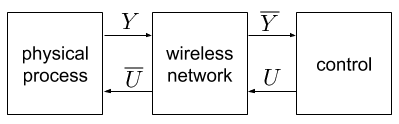
\includegraphics[width=0.95\columnwidth]{diagrams/fbd-system}
	\caption{Functional block diagram of a cyber-physical system in which a physical process and an automation system interact through a wireless network.}
	\label{fig:fbd-system}
\end{figure}

An alternative to schematic diagrams is SysML~\cite{SysML2017}. SysML is a general purpose modeling language that is often used for model-based systems engineering (MBSE) practice within industrial systems~\cite{MBSEandSysML}. SysML provides structural, behavioral, and parametric semantics for the analysis of complex systems. For examples, systems analysis using SysML enables capturing and communicating system requirements and design which include hardware, software, firmware, information flows, and processes with graphical notations. Within the factory automation industry, engineers are adopting SysML in the form of MBSE to develop realizable operational models of the factory and data flow processes. MBSE models address verification of design through executable simulations depending on the modeling tool.  The SysML specification is defined in~\cite{SysML2017}.  In SysML, the basic semantic constructs of the language are Packages, Blocks, Ports, Interfaces, and Constraints, in addition to the constructs provided by the Unified Modeling Language (UML). Packages are logical grouping of model elements. Package relationships are captured using the package diagram (PKG). Relationships of these constructs are captured in the block definition diagram (BDD).  The internal composition and connectivity of parts are captured in the internal block diagram (IBD). SysML includes other types of diagrams and semantic constructs that are not required for this analysis and are not explained here. The SysML model is comprehensive; however, the size and number of diagrams within the model are too extensive to include within this paper.  Therefore, the reader is encouraged to explore the SysML model defined in~\cite{SysML.Candell2018}.  A useful primer on SysML may be found in~\cite{Friedenthal2015.SysML}. 

Examples of the use cases and methodologies of using different graphical models for the analysis of manufacturing systems are explored in~\cite{Lutjen2015.GramosaMethod,Luder2011.GraphicalModeling,Jia2013.GraphicalModeling,Alvarez2013.GraphicalModeling}.  In~\cite{Quinsat2017.SysML}, SysML is used to capture both composition and behavior of an additive manufacturing work-cell.  A survey of applying graphical modeling languages in capturing information flows within a product service system which may be applied to manufacturing enterprises~\cite{Durugbo2011.GraphicalModeling}.  Our approach compliments these previous examples by combining the operational and wireless information transport systems together in a single model, thereby facilitating a single model that may be used for simulation and other systems engineering analyses.

While various architectures for the work-cell exist as exemplified in the literature, a common language and framework for communicating architecture and information flow has not been established for cross-domain interactions between the manufacturing system and its supporting communication networks.
SysML contains the semantics for such engineering capture and provides an industry accepted language for communicating composition, interfaces, and information flow. Moreover, SysML provides the semantics for assigning properties to any model element such that those properties are made  available for analysis using other tools such as Prot\'eg\'e \cite{StanfordUniversity.Protege} and the Web Ontology Language (OWL) \cite{W3C2012.OWL}.
It is important to understand that while SysML provides semantics for a formal capture of architecture, information flow, and parametric constraints, it may also be used for a higher-degree of abstraction provided by the functional block diagrams.  

\section{Conceptual Representation} \label{sec:conceptual}
The remainder of this work describes a reusable model for representing a comprehensive wireless factory work-cell using the semantic constructs of SysML.  We now follow with an exposition of our model beginning with the conceptual model followed by a detailed description of each component within the model. When discussing the model, the SysML term, \textit{block}, is omitted for the sake of brevity where the meaning is clear. 
\subsection{Packages}
The factory work-cell is decomposed into one general and nine major structural packages as shown in Fig.~\ref{fig:pdd-workcell}.  Packages include major logical groupings of structure within the model.  These packages are enumerated in the following paragraphs.

\begin{figure}[t]
	\begin{center}
		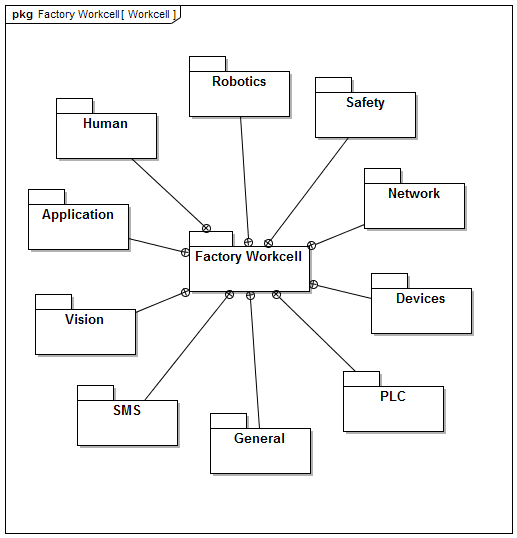
\includegraphics[width=0.95\columnwidth]{diagrams/pkg__Factory_Workcell__Workcell}%
		\caption{SysML package diagram showing the logical containment of the factory work-cell structural elements.}%
		\label{fig:pdd-workcell}
	\end{center}
\end{figure}


\subsubsection{General} A set of reusable structural elements that is used for conceptual modeling or extended to produce more complex model elements.  Each of the sub-packages within the General package extends basic features.  The sub-packages within General include time and constraints for data, electro-magnetics, and motion.

\subsubsection{Network} Describes the components, blocks, interfaces, and limiting factors of the industrial wireless network (IWN).  The IWN is modeled as the radio channel and the services provided by the network. Limiting factors are modeled as parametric equations associated with the radio channel and the services.

\subsubsection{Application}  This package contains the model elements describing a component of behavioral functionality typically implemented within software or firmware but could be implemented in hardware.  It describes the features and constraints of factory operation such as the logic of a supervisory controller or the feedback controller of a robot arm.  The Application sets the performance requirements of the wireless network, i.e., the factory network performance requirements are derived from the requirements of the applications deployed to a work-cell.

\subsubsection{Devices} Describes the types of devices found within the factory work-cell to include any device that interacts with the environment such as wired and wireless input-output (IO) devices including sensors and actuators.

\subsubsection{Robotics} Describes the computational and communicative components of robot control including sensing, actuation, and command.  Description of the robot itself is inconsequential to communication and therefore not included in the model.

\subsubsection{PLC} Describes the supervisory control components commonly handled by one or more programmable logic controller (PLC) components.  This package includes the elements responsible for coordination of actors and handling of most input-output.

\subsubsection{Safety} Describes the allocation of safety qualities typically included in the supervisory controller.  The Safety package includes devices, monitoring, and actuation of the safety behaviors within the factory work-cell.

\subsubsection{Vision} Describes the allocation of features to optical monitoring and tracking which are typical to the collaborative robotic work-cell.

\subsubsection{Spectrum Monitoring System (SMS)} Describes the qualities and interfaces of a factory spectrum monitoring system projected into the factory work-cell.  The SMS includes monitoring nodes and agents localized to the work-cell and connected to the automation system for real-time adaptation to changing multi-path and interference. 

\subsubsection{Human} Describes the features associated with human beings such as human motion, tasks, and carried equipment such as portable computing and communication devices.
\vspace{3mm} 

Several examples of how to use the model are provided within the model\cite{SysML.Candell2018}.  Examples include: a robotic force-torque leader-follower, a robotic force-torque limiter, a collision avoidance, and a robotic pick and place work-cell.  The parametric constraints are provided as examples and are intended to be used for communication to project stakeholders or replaced with executable computer code such as MATLAB or Python scripts, thereby making the model useful for simulation depending on the modeling tool selected.

\begin{figure*}
	\centering
	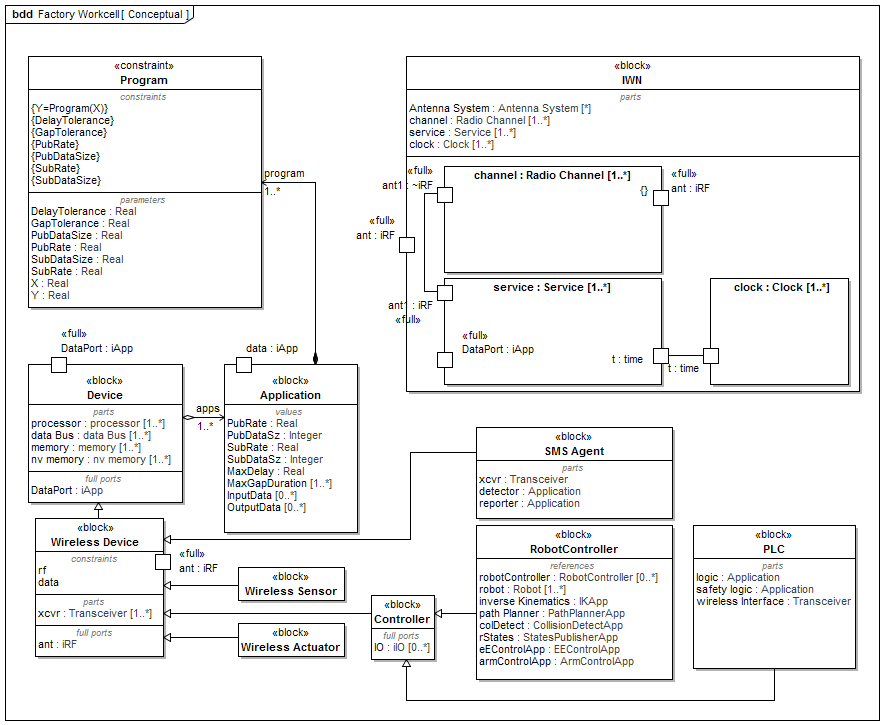
\includegraphics[width=0.97\textwidth]{diagrams/bdd__Factory_Workcell__Conceptual}%
	\caption{Architecture of the conceptual work-cell captured as a SysML block definition diagram.  In this diagram, only the most generalized blocks necessary to construct a work-cell scenario are shown.  More application-specific scenarios may be developed by deriving new blocks from the constructs shown here. The shapes and connectors used for expressing this model are defined in the SysML specification\cite{SysML2017}. }%
	\label{fig:conceptual:bdd}
\end{figure*}

\subsection{Conceptual Architecture}\label{sec:architecture}
The conceptual architecture of the wireless work-cell model is depicted in Fig.~\ref{fig:conceptual:bdd}. All the packages are included in this architecture, and the connections and relations between blocks are defined using the SysML semantics. This figure serves to orient the reader during the presentation of detailed model decomposition in Section~\ref{sec:detailed-model}. The work-cell model is composed of at least one Industrial Wireless Network (IWN) block and at least one Device block. More IWN blocks are used when multiple wireless networks coexist within the industrial work-cell. Applications are associated with Devices and performance constraints are applied to Applications. In this model, the Wireless Device is a subclass of Device, and the Controller is a further derivation of the wireless device. Moreover, the Controller is an abstract specialization of a wireless device that represents all types of devices intended to control other processes. The behaviour of a PLC or Robot is represented through two packages in the model. The production related behaviour is represented through the corresponding packages and the connectivity behaviour is represented through Devices such as the Robot Controller and the PLC which are special classes of Wireless Device containing all of the structure and behavior of the wireless device. Finally, an often overlooked component of any industrial wireless deployment is the spectrum monitoring system represented by the SMS Agent. Blocks in the model communicate through ports such as the \textit{ant} port which represents the antenna or waveguide interface.  Composition is further implied by the parts, constraints, and parameters associated with each block. These are listed within the compartments of each block.

\section{Detailed Model Decomposition}\label{sec:detailed-model}
In this section, we describe in detail the decomposition of the model packages. The decomposition of each package includes the properties and the components of the package where the relation between the package and physical industrial work-cells is illustrated. Moreover, some of the packages may have various types with different properties and hence sub-packages are defined for these packages. This section also includes a general explanation of the packages rules in the work-cell and the behavioral interactions between the packages.      

\subsection{General Package}
The General package contains the reusable elements of the model.  In particular, the General package contains elements that are not particular to any one work-cell component but can be reused or applied across several.  The concepts of time, clocks, and synchronization are included within General.  Moreover, several types of constraints are defined.  

\subsubsection{Time}
Time is an important construct within communication systems as well as industrial control systems.  Time is realized as a set of one or more clocks. A work-cell will contain one to several clocks typically embedded within each device to allow those devices to synchronize to a common clock. The local clocks within the work-cell devices will synchronize to a master reference clock and usually one with a high degree of precision, accuracy, and stability.  The degree to which the local clocks synchronize to the master will depend on the requirements of the applications that the local clocks serve.  Clock synchronization can be costly in power, size, and monetary cost of the devices, but it may be necessary depending on the applications using a clock.  Clock performance is a key driver of size and power consumption, and synchronization of clocks across a wireless network can be a challenge and is a highly studied field~\cite{ClockSync.Mahmood2017,ClockSync.Geetha2017}. Moreover, the Time package includes a constraint, Clock Performance, to represent the production of time and synchronization with a master clock. 

\subsubsection{Constraints}\label{sec:general:constraints}
Constraints provide limitations on the performance of an element within the model.  Within General, several constraints are defined which may be applied to any block within the model. These constraints include motion constraints, radio channel constraints, and networking constraints as shown in Fig.~\ref{fig:constraints:motion}-\ref{fig:constraints:network}.  

\paragraph{Motion Constraints}\label{sec:constraints:motion}

\begin{figure}[tbp]
	\centering
	\subfloat[Motion Constraints\label{fig:constraints:motion}]{%
		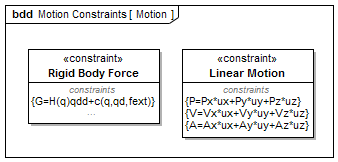
\includegraphics[width=0.95\columnwidth]{diagrams/bdd__Motion_Constraints__Motion}}
	\hfill
	\subfloat[Radio Channel Constraints\label{fig:constraints:radio}]{%
		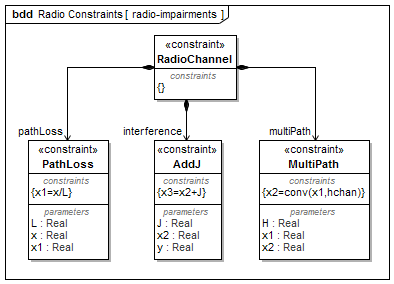
\includegraphics[width=0.95\columnwidth]{diagrams/bdd__Radio_Constraints__radio-impairments}}
	\hfill
	\subfloat[Networking Service Constraints\label{fig:constraints:network}]{%
		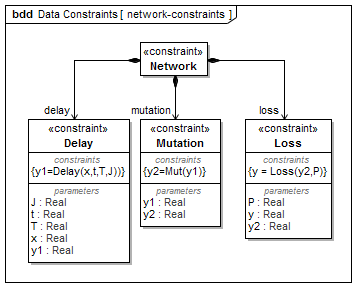
\includegraphics[width=0.95\columnwidth]{diagrams/bdd__Data_Constraints__network-constraints}
	}  
	\caption{Generalized network constraints consisting of rigid body motion~\protect\subref{fig:constraints:motion}, the radio channel~\protect\subref{fig:constraints:radio} and the network services~\protect\subref{fig:constraints:network}.}
	\label{fig:general:constraints}      
\end{figure}

When applied, these constraints provide the bounds of dynamical performance.  For example, motion constraints determine the positions, velocities, and accelerations on a rigid body.  The force vector equations \eqref{eq:robot:dynamics} are the general governing dynamic laws of motion as forces on a vector of joints as exerted by the end-effector or set of end-effectors on the environment.  The equations constrain the robot to operate according to the laws of physics, where the joint-space inertia matrix, $H$, is an ${n}\times{n}$ symmetric, positive-definite matrix, and $q$, $\dot{q}$, and $\ddot{q}$ are vectors of position, velocity, and acceleration, respectively.  The variable $f_{ext}$ is the six degrees of freedom (DOF) force acting on the end-effector, and $c$ is the joint-space bias force required to produce a zero sum force on the end-effector~\cite{Featherstone2007}.  
\begin{equation}
\label{eq:robot:dynamics}
\Gamma = H(q) \ddot{q} + c(q,\dot{q},f_{\!ext})
\end{equation}    
where $\Gamma$ is the vector of forces exerted by the end-effectors.  

This system of equations is controlled using a combination of digital feed-forward and feedback compensation in which the communication mechanism of the robot states directly impacts the controller's effectiveness. Joint control via a wireless network connection is typically avoided; however, monitoring of the linear and angular forces represented by $f_{\!ext}$ as sensed by a 6-DOF force-torque (FT) wireless sensor can be advantageous for many industrial applications.  As such, the performance of the wireless connection between a FT sensor and the controller can be a limiting factor in the performance of force-sensitive applications. Such a constraint may be applied to robot manipulators as defined in Section~\ref{sec:robotics}.

\paragraph{Radio Channel Constraint}\label{sec:constraints:radio}

The radio channel constraint limits wireless information flow to the laws of propagation which includes path loss, reflection, diffraction, and interference.  By applying this constraint to Wireless Devices described in Section~\ref{sec:devices:wireless-device}, such devices experience the effects of a lossy communication medium. The radio channel when applied to a wireless communication link within the work-cell manifests itself in accordance of the illustration of Fig.~\ref{fig:par:iwn-radio}.  The parametric equations for the radio channel include path loss, multi-path, and interference.  Path loss is generically modeled as the input signal divided by the bulk power loss in the channel. Path loss is often characterized as a two-piece linear function of distance\cite{Candell2017.NIST1951}. Multi-path is modeled as convolution of the transmitted radio signal with a linear time-varying impulse response characterizing the electromagnetic propagation between transmitter and receiver antenna systems.  Interference is then modeled as an additive component with power, bandwidth, and probability of excitation.

\begin{figure}[tbp]
	\centering
	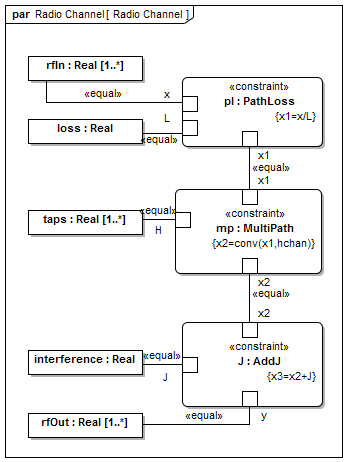
\includegraphics[width=0.95\columnwidth]{diagrams/par__Radio_Channel__Radio_Channel}%
	\caption{SysML parametric diagram of the radio channel constraints of the industrial wireless network.}%
	\label{fig:par:iwn-radio}
\end{figure} 

\paragraph{Data Constraints}\label{sec:constraints:data}

\begin{figure}[tbp]
	\centering
	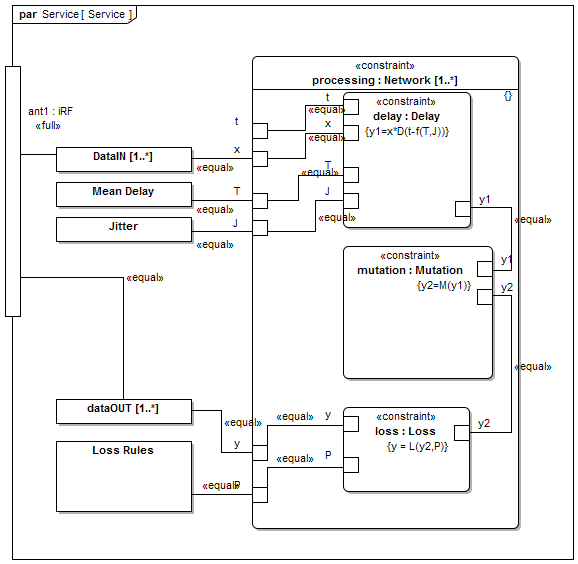
\includegraphics[width=0.95\columnwidth]{diagrams/par__Service__Service}%
	\caption{SysML parametric diagram of the data constraints applied to the industrial wireless network.}%
	\label{fig:par:iwn:data}
\end{figure}    

Delay, mutation, and loss of information within the industrial wireless network are encapsulated by the Network constraints block.  The Network constraint is applied to wireless devices within the network and represents the impacts of the radio channel and network components and protocols.  These constraints are illustrated in a parametric diagram of Fig.~\ref{fig:par:iwn:data} in which the rules for delay, mutation, and loss are applied to a service of an industrial wireless network within a work-cell. As with any constraint, the rules for data loss may be modeled as equations, psuedocode, or executable computer code such as MATLAB script or C.  These rules decide if information is lost due to delay or mutation.  While it is easy to understand how mutation leads to loss through a mechanism such as a checksum, unacceptable delay can also lead to loss of data.  

% equations for data constraints
Delay is simply a function of time, the physical environment of the factory work-cell, and state of the network at time, $t$. Many features of the network and the physical environment will have an impact on the output of the delay equation and will include data transmission duration, radio wave propagation delay, signal-to-noise, protocol for reliability, routing, internal queuing, and processing. A generalized equation for information delay by the wireless network is given as the sum of processing delay, queuing delay, transmission delay, and propagation delay. Subsequently, information loss is modeled as a set of rules governed by the attributes of the network infrastructure, transport medium, and protocols shown in~\eqref{eq:network-loss}. These rules may include thresholds for unacceptable delay and the ability of the network to correct for data mutation or loss in the physical channel (i.e. the air interface).

\begin{equation}\label{eq:network-loss}
\mathcal{Y}(t,\mathcal{X},\mathcal{N}) = 
\begin{cases} 
\mathcal{X} & \text{if } \mathcal{X} \vdash \mathcal{L}(t,\mathcal{X},\mathcal{N}) \\
\emptyset   & \text{otherwise}
\end{cases}
\end{equation}
where $\mathcal{X}$ and $\mathcal{Y}$ are blocks of data traversing the network and $\mathcal{N}$ is the state of the network at time, $t$.	We model the loss constraints as a general set of rules, $\mathcal{L}$, taking into account that each network system will have a different set of configuration attributes and protocols.  The rules will therefore change for each operational system and the networks used.  When the rules for loss are applied, the output of the network, $\mathcal{Y}$, becomes the input to the network, $\mathcal{X}$, when $\mathcal{X}$ satisfies $\mathcal{L}(t,\mathcal{X},\mathcal{N})$.

\subsection{Application}\label{sec:application}

\begin{figure}[tbp]
	\centering
	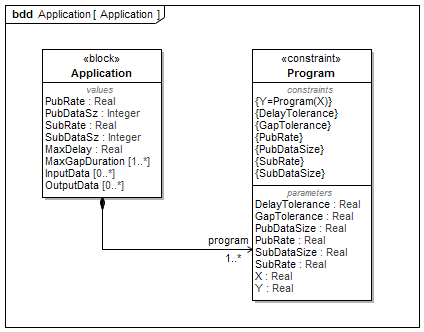
\includegraphics[width=0.95\columnwidth]{diagrams/bdd__Application__Application}
	\caption{Block definition diagram of the Application.}
	\label{fig:application:bdd}
\end{figure}

Applications, commonly implemented as software and firm-ware, represent the intelligence of devices. The application defines the behavior and the information flow requirements of the work-cell~\cite{appWorkcell1996, appWorkcell2001, appWorkcell2011}.  As defined in the model, without Applications implemented in software, firmware, or hardware, the work-cell devices would not function.  The definition of the Application block is shown in Fig.~\ref{fig:application:bdd}.  The Application block is constrained by the Program constraint which defines the logic of the program, its expected data flow input rates, and its tolerances to delay and information loss.  Devices host multiple applications each with a unique set of constraint properties.  It is essential when constructing a work-cell model that each application is identified and modeled appropriately.  An example of an Application is a collision detection system within a robot controller. Table~\ref{tab:sample:constraints} illustrates sample parameters used in the collision detector Application.

% 	\vbox{%
% 		\begin{description}[align=left, labelindent=5mm]
% 			\label{fig:CollDet:example}
% 			\item [Program] Collision Detector
% 			\item [Constraints] ~
% 			\begin{description}[align=left]
% 				\item[Input Data] robot states, 1 KB
% 				\item[Subscription Rate] robot states, 125 \si{\Hz}
% 				\item[Max Delay Tol.] robot states, 47 \si{\us}
% 				\item[Max Loss Duration] robot states, 275 \si{\ms}
% 			\end{description}
% 		\end{description}
% 	}

\begin{table}[tbp]
	\caption{Constraints Pertaining to a Collision Detector} \label{tab:sample:constraints}
	% Table generated by Excel2LaTeX from sheet 'constraints'
	\begin{tabular}{lc}
		
		\textbf{Constraint Property} &
		\textbf{Typical Value}
		\\
		\midrule
		Input Payload Size &
		1 KB
		\\
		Subscription rate &
		125 Hz
		\\
		Maximum Delay Tolerance &
		47 $\mu$s
		\\
		Maximum Loss Duration &
		275 ms
		\\
	\end{tabular}%
	
\end{table}

Specification of Application constraints provides a clear picture of the requirements of the factory automation system which can be projected on the wireless network. Through this process, it is possible to determine such requirements as scalability, throughput, reliability, and latency of the supporting network services modeled as radio and data constraints in Section~\ref{sec:general:constraints}. Indeed, as the manufacturing system becomes more complex and wireless becomes essential to communication, the projection of manufacturing requirements onto the wireless communication system becomes less clear.  Frequency planning, transmission scheduling, and error correction schemes become less obvious, and considerations of power, reliability, latency, and scale become optimization trade-offs. Such analyses are not within the scope of this paper but are important considerations for future research of manufacturing systems.  As such, the architectural elements and information flows exposed by an abstract model are a necessary first step.

\subsection{Industrial Wireless Network}

Central to the automation system is connectivity among devices and controllers~\cite{controlWSAN2010}.  More specifically, modern automation systems often employ networks to conduct inter-device communication~\cite{wirelessAutomation2017}.  The term \textit{inter-device} is appropriate as the Device block serves as the basis for all other components that communicate through the network.  Our model of the IWN is composed simply as a radio channel, a set of services, and a set of clocks as shown in Fig.~\ref{fig:iwn:bdd}.  This simplification of the model is necessary to allow the users of the model to provide as much or as little detail of the implementations of the radio channel and underlying services as required for their implementations.

\begin{figure}[tbp]
	\centering
	\subfloat[\label{fig:iwn:bdd}]{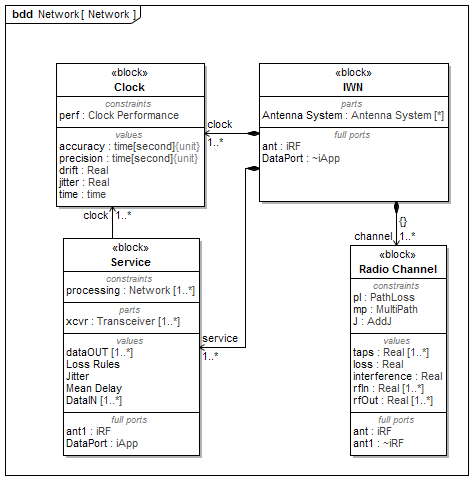
\includegraphics[width=0.99\columnwidth]{diagrams/bdd__Network__Network}}
	\hfill
	\subfloat[\label{fig:iwn:ibd}]
	{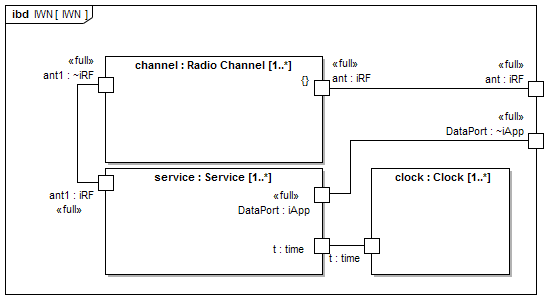
\includegraphics[width=0.99\columnwidth]{diagrams/ibd__IWN__IWN}}
	\hfill
	\subfloat[\label{fig:iwn-services:ibd}]
	{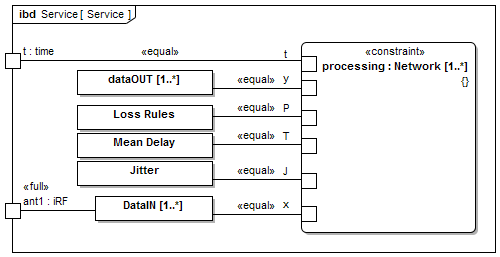
\includegraphics[width=0.99\columnwidth]{diagrams/ibd__Service__Service}}\\
	\caption{The BDD~\protect\subref{fig:iwn:bdd} and IBD~\protect\subref{fig:iwn:ibd} of the industrial wireless network with parametric IBD~\protect\subref{fig:iwn-services:ibd} of the Services block.}
	\label{fig:iwn:ibd:full}
\end{figure}

Connectivity of a constructed IWN is shown in Fig.~\ref{fig:iwn:ibd}.  An IWN is internally modeled such that information flows as radio frequency (RF) energy through the \textit{ant} port.  A radio channel is applied, theoretically for each pairwise link, and the modified signal is passed to the services for processing.  Network processing is modeled by the properties of network constraints as defined in Section~\ref{sec:constraints:data}.  Once processed by network services, information is routed back through the radio channel through the \textit{ant} port to other Devices connected to the IWN.  Moreover, the Service block includes a parametric model as shown in Fig.~\ref{fig:iwn:ibd:full}. This IBD with exposed parametrics exemplifies the inclusion parameters such as information delay and loss caused by the IWN, but it also exemplifies the impact of protocols and infrastructure (throughput, memory, etc.) within the network.  These effects are modeled as rules of loss shown in~\eqref{eq:network-loss}.

\subsection{Devices}\label{sec:devices}

\subsubsection{Device}\label{sec:devices:device}

A Device, defined in Fig.~\ref{fig:bdd:devices}, is generic construct representing an element within the work-cell with processing, memory, and storage capability. Devices have the capability to run applications as defined in Section~\ref{sec:application}.  Devices are sub-classed into Sensor and Actuator devices which generically refer to any type of sensor or actuator, and, in particular, the wired variety.  The Device is further sub-classed to the Wireless Device which is the central theme of our analysis.  Derived from the Wired Device are the Wireless Sensor and Wireless Actuator as well as the Controller.  The Controller represents the base class for deriving work-cell devices such as the PLC and the Robot Controller, sections~\ref{sec:plc} and~\ref{sec:robotics}, respectively, and provides support for external input-output (IO).

\begin{figure}[H]
	\centering
	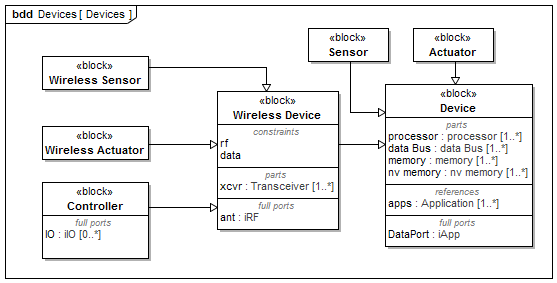
\includegraphics[width=0.95\columnwidth]{diagrams/bdd__Devices__Devices}%
	\caption{SysML block definition diagram of wireless devices within the factory work-cell.}%
	\label{fig:bdd:devices}
\end{figure}



\subsubsection{Wireless Devices}\label{sec:devices:wireless-device} 
A Wireless Device is a subclass of Device that contains the various components necessary for untethered communication.  These devices then communicate with each other through one or more industrial wireless networks (IWNs) which contains antenna systems, transceivers, protocols, and network services.  The relationships and composition of the Wireless Device are illustrated in Fig.~\ref{fig:wirelessdevice:full}. As shown, the wireless device is composed of at least one transceiver and each transceiver is composed of at least one antenna system which is composed of at least one antenna element.  The antenna system is constrained by its gain profile.

\begin{figure}[tbp]
	\centering
	\subfloat[Block definition diagram of the Wireless Device\label{fig:wirelessdevice:bdd}]{%
		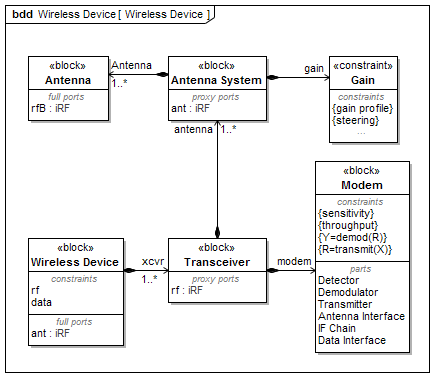
\includegraphics[width=0.95\columnwidth]{diagrams/bdd__Wireless_Device__Wireless_Device}
	}
	\hfill
	\subfloat[Internal block diagram of the Wireless Device\label{fig:wirelessdevice:ibd}]{%
		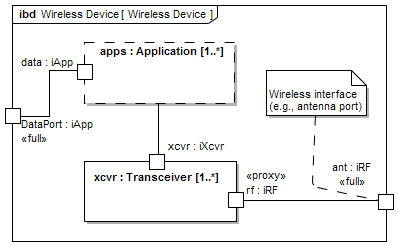
\includegraphics[width=0.95\columnwidth]{diagrams/ibd__Wireless_Device__Wireless_Device}
	}  
	\caption{Block definition diagram~\protect\subref{fig:wirelessdevice:bdd} and the internal block diagram~\protect\subref{fig:wirelessdevice:ibd} of Wireless Device.}
	\label{fig:wirelessdevice:full}      
\end{figure}

\subsubsection{Test Device}\label{sec:test-device}

\begin{figure}[tbp]
	\centering
	\subfloat[Block definition diagram of the Test Device\label{fig:testdevice:bdd}]{%
		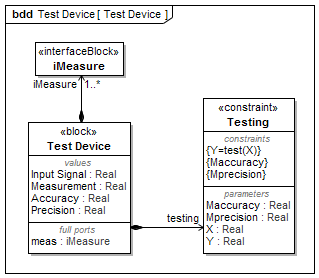
\includegraphics[width=0.95\columnwidth]{diagrams/bdd__Test_Device__Test_Device}
	}
	\hfill
	\subfloat[Internal block diagram of the Test Device\label{fig:testdevice:ibd}]{%
		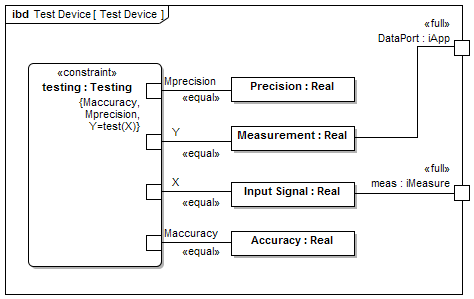
\includegraphics[width=0.95\columnwidth]{diagrams/ibd__Test_Device__Test_Device}
	}  
	\caption{Block definition diagram~\protect\subref{fig:testdevice:bdd} and the internal block diagram~\protect\subref{fig:testdevice:ibd} of Test Device.}
	\label{fig:testdevice:full}      
\end{figure}

The Test Device is a subclass of Device that represents devices used for calibration or ground truth testing of properties of a work-cell.  The block definition and internal configuration are illustrated in Fig.~\ref{fig:testdevice:full}.  A Test Device is constrained by its accuracy and precision as well as the algorithm for controlling measurement.  An example of a test device is a calibrated force sensor that may be used as comparison to a 6-DOF wireless sensor mounted on the wrist of a robot arm as shown in the top left of Fig.~\ref{fig:workcell:examples}. Test devices are useful and necessary elements of the wireless testbed to establish accurate and repeatable ground truth measurements.  For example, a stationary precision force sensor may be used to establish a ground truth force value, and a high-accuracy vision tracking system is used for truth in position.  Test devices are modeled such that measurements may traverse the operational wireless network or a stand-alone wired interface.

\subsection{Robotics}\label{sec:robotics}
\begin{figure}[tbp]
	\centering
	\subfloat[Block definition diagram of the Robot Controller\label{fig:robotcontroller:bdd}]{%
		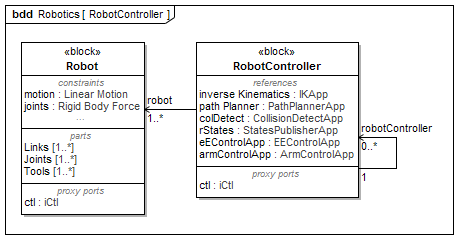
\includegraphics[width=0.95\columnwidth]{diagrams/bdd__Robotics__RobotController}
	}
	\hfill
	\subfloat[Internal block diagram of the Robot Controller\label{fig:robotcontroller:ibd}]{%
		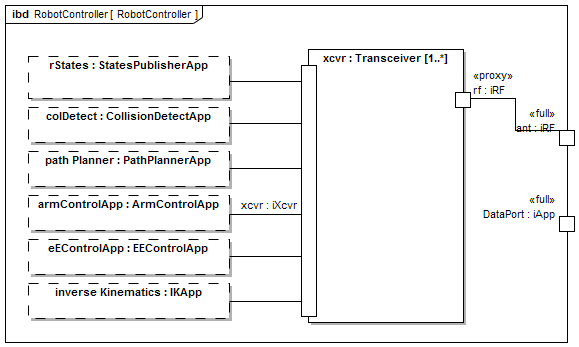
\includegraphics[width=0.95\columnwidth]{diagrams/ibd__RobotController__RobotController}
	}  
	\caption{The BDD~\protect\subref{fig:robotcontroller:bdd}, IBD~\protect\subref{fig:robotcontroller:ibd} of the Robot Controller.}
	\label{fig:robotocontroller:full}	
\end{figure}

The robotics package contains elements specific to robot systems.  Robot systems are composed of at least one robot controller associated with one or more robots, as shown in Fig.~\ref{fig:robotcontroller:bdd}.  In manufacturing, robots interact with their surrounding to accomplish assigned tasks such as tending machinery, moving materials, welding, and inspecting. Robot controllers provide support for external IO devices.  In addition, modern robot controllers will support a variety of open and proprietary network protocols allowing for interaction with other actors in the work-cell.  The robot controller's main task is control of the rigid body dynamics of the robots which is usually conducted via real-time communication over a high-throughput serial field-bus. While joint control is conducted using wires, the robot controller is responsible for other tasks requiring reliable, low-latency communication in which wireless may serve a role.  These tasks are captured in the model as applications (Fig.~\ref{fig:robotcontroller:ibd}) and explained as follows.

\begin{description}
	
	\item[\textbf{Robot States Publisher}] Transmission of robot states to external actors such as other robot controllers, supervisors, and safety systems.
	
	\item[\textbf{Arm Controller}] Also known as manipulator control, serves to accept position commands as Cartesian or joint space trajectories and waypoints from other actors within the work-cell.
	
	\item[\textbf{End Effector Control}] Command and control of the robot end-effector such as a gripper or sensor.  The end-effector may be equipped with a high-throughput wireless sensor necessitating reliable communication.
	
	\item[\textbf{Inverse Kinematics}] Converts Cartesian coordinates of the end-effector into joint positions.
	
	\item[\textbf{Path Planner}] Determines the optimal geometrical trajectory to achieve a final pose given knowledge of self-collision and real-time knowledge of the surround environment.  Path planning is a sophisticated part of a robot system and may be allocated to an external system depending on throughput and latency requirements.
	
	\item[\textbf{Collision Detector}] This application monitors the states of other actors and obstructions within the work-cell. If possibility of collision is detected, the collision detector takes action.
	
\end{description} 

These applications within the robotic work-cell define many information flows requiring careful analysis to achieve reliability and latency necessary for the safety and control of the manufacturing process. Information flows are identified in Section~\ref{sec:wireless-infoflows}.

\subsection{PLC}\label{sec:plc}
The PLC is a specialized class of Controller.  PLCs were originally developed to mirror relay circuits in software; however, the modern PLC is much more advanced and is usually equipped with multiple processors, a real-time operating system (OS), and capabilities to support various types of industrial IO devices.  In addition, modern PLCs (also called automation servers) include both a general purpose OS with a real-time kernel and multiple network interfaces.  Many network-routable protocols are also supported.  With the addition of wireless protocols, PLCs now have the ability to support IO devices connected remotely without wires.  Supervision of untethered robots is also possible using PLCs.  The PLC is modeled as a Controller device with the work-cell model.  Shown in Fig.~\ref{fig:PLC:ibd}, the PLC is modeled as a wireless device with transceiver, logic application, and safety applications.  More sophisticated PLCs may be modeled by extending the PLC block.  As applications, the logic and safety functions are constrained by application constraints. Finally, as Controller devices, PLCs are modeled with an IO port, thus IO can be connected to the PLC by wires or by wireless network connection.

\begin{figure}
	\centering
	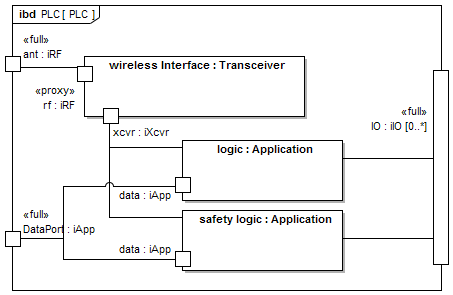
\includegraphics[width=0.95\columnwidth]{diagrams/ibd__PLC__PLC}
	\caption{The IBD of the PLC showing composition and connectivity of the control logic and safety logic Application instantiations to the Transceiver interface. }
	\label{fig:PLC:ibd}
\end{figure}

\subsection{Safety}\label{sec:safety}
% 	\textcolor{red}{MOHAMED TO WRITE}
% 	\textcolor{blue}{Allocation of safety features from the PLC. High availability IO input devices, output relays, used for E-STOP usually to protect life and property; constrained by response time requirement of the safety rating}

In a work-cell with interacting humans and robots, functional safety requirements are typically strict by specifying the rules related to four main safety criteria, namely, monitored stops, controlled speeds, separation distances, and power and force limits in order to prevent injury for humans and damage for equipment. The wireless safety package is composed of a safety controller and safety devices. Traditionally, the safety requirements of the work-cell is fixed and managed by the safety controller which receives safety-related measurements and takes the corresponding actions. Alternatively, the safety controller may be connected to the PLC where the current work-cell activities are supervised.  The PLC will determine the required safety rating and the safety controller behaves accordingly. The dedicated safety controller is needed to achieve the required high reliability and low latency safety requirements and it can be a general PLC with safety modules. 

The safety devices include non-safety-rated devices such as the various work-cell sensors and actuators and safety-rated input and output devices. Safety control input devices include Emergency-stop and enabling buttons while output devices include relays and switches for various work-cell equipment. The use of wireless in safety control loops allows installing a larger number of sensing devices including vision systems to monitor the human and robots activities, velocity and proximity sensors, and machine status sensors. Moreover, wireless allows to have mobile control panels where workers can activate a safety device at any time and location within the work-cell.        

\subsection{Vision}\label{sec:vision}
% 	\textcolor{red}{MOHAMED TO WRITE}
% 	\textcolor{blue}{composition (vision processing, optical devices with networking interfaces, general panning and zooming, object detection, interface to robotic system, interface to the supervisory system)}

%     \textcolor{green}{Make that we allow the following in your definition: part tracking, object detection, intput to collision avoidance systems, tracking of mobile robots, augmented reality devices/systems, security cameras, etc.}
The vision system considered in this subsection is the one used for work-cell monitoring and general object detection. It does not cover the machine-embedded vision systems which can be used for inspection and characterization of objects such as the shape, color, texture, or size of processed materials. The data collected by the work-cell vision system can be used for parts and mobile robots tracking, collision avoidance, object detection, security identification systems, and augmented reality devices and systems. The vision system communicates with the supervisory control, robotic controller, and the safety system to provide the work-cell state which contains the positions of various equipment, robots, and humans. 

The vision system is composed of optical devices, vision processing unit, and interfaces to various work-cell systems. The optical devices are the cameras for capturing images at high enough speed to track and detect various objects. These cameras have wireless network interfaces to be connected to the vision processing unit to allow collaborative processing of the captured images and obtaining precise work-cell state. The vision processing unit performs data acquisition from the distributed optical devices and feature extraction to detect and track the positions of various entities in the work-cell. 

The vision system communicates the corresponding data to the supervisory control, robotic control, and the safety system for decision making based on the captured work-cell state. The supervisory controller uses vision system data for robots and workers localization, parts detection and identification, and schedules tasks using this information. The robotics controller uses these data for motion control, path planning, and collision detection. Finally, the safety controller uses these data for safety requirements implementation such as enforcing safety stops, controlling the speeds of moving objects, and limiting power and forces of various work-cell components.    

\subsection{Spectrum Monitoring System}\label{sec:sms}
A spectrum monitoring system (SMS) is an often overlooked yet valuable part of the wireless factory work-cell with requirements specified in~\cite{Candell2017.SMS}.  The SMS is modeled as an atomic agent within the work-cell.  The SMS Agent is one component in a larger enterprise-level spectrum monitoring deployment.  The SMS agent shown in Fig.~\ref{fig:sms:bdd} includes a transceiver, an event detector, and a reporting agent.  The transceiver can be implemented as an RF-to-baseband converter.  The detector application is responsible for detection and estimation of anomalous spectral events and may employ machine learning to accurately detect anomalies and report localized spectral events.

The reporter application collects, filters, and reports event information to a central management console.  SMS reports support identification of long-term patterns such as growth trends in particular wireless bands.  Since the SMS Agent is part of a larger network of spectrum monitoring, it is presumed that reports are wirelessly transmitted back to the enterprise management console.  These reporting events use bandwidth otherwise used for the factory operation, thus reports must be made concise and infrequent.  This implies substantial filtering and intelligence in the local SMS agents This may provide opportunities for research.

Detection events may be routed to the local supervisor, robot controller, and safety system.  By leveraging spectral awareness, work-cells can be made safer and more reliable.  As SMS are not yet widespread in industrial applications; thus, standardized protocols are needed for reporting and integration with automation systems.

\begin{figure}[tbp]
	\centering
	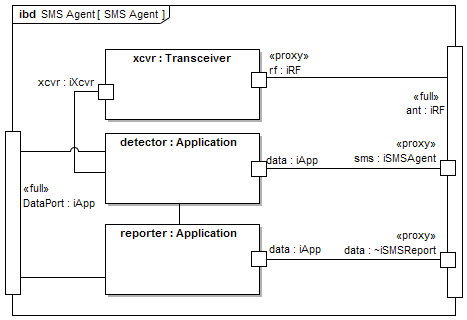
\includegraphics[width=0.99\columnwidth]{diagrams/ibd__SMS_Agent__SMS_Agent}
	\caption{Spectrum monitoring agent composed of transceiver, detection application, and reporting application.}
	\label{fig:sms:bdd}
\end{figure}

\subsection{Human}\label{sec:human}
% 	\textcolor{red}{Mohamed to write}
% 	\textcolor{blue}{People; wearable devices such as gas sensors, identification, and localization; could be security related for access control; portable devices; personal devices; include motion on factory floor; operational tasks; intervention of process      
% 		Composition, constraints of motion}

Humans can exist in a modern work-cell for short or long periods of time depending on the required task. Two categories of human-related aspects are captured in the work-cell model. First, the human existence in the work-cell leads to detection and identification of the corresponding worker for both safety and security. Also, human motion within the work-cell requires position tracking for environment monitoring and spectrum monitoring due to radio frequency channel variations with human movements. The second category includes the human interfaces with the work-cell process that include portable control devices, wearable sensors, and workers communication devices to get task commands. Moreover, depending on the process constraint, personal devices of workers may interfere with the work-cell communications if allowed.      

\section{Results of a Work-cell Case Study}\label{sec:wireless-infoflows}
% Rick's section	
\begin{figure*}[tbp]
	\centering
	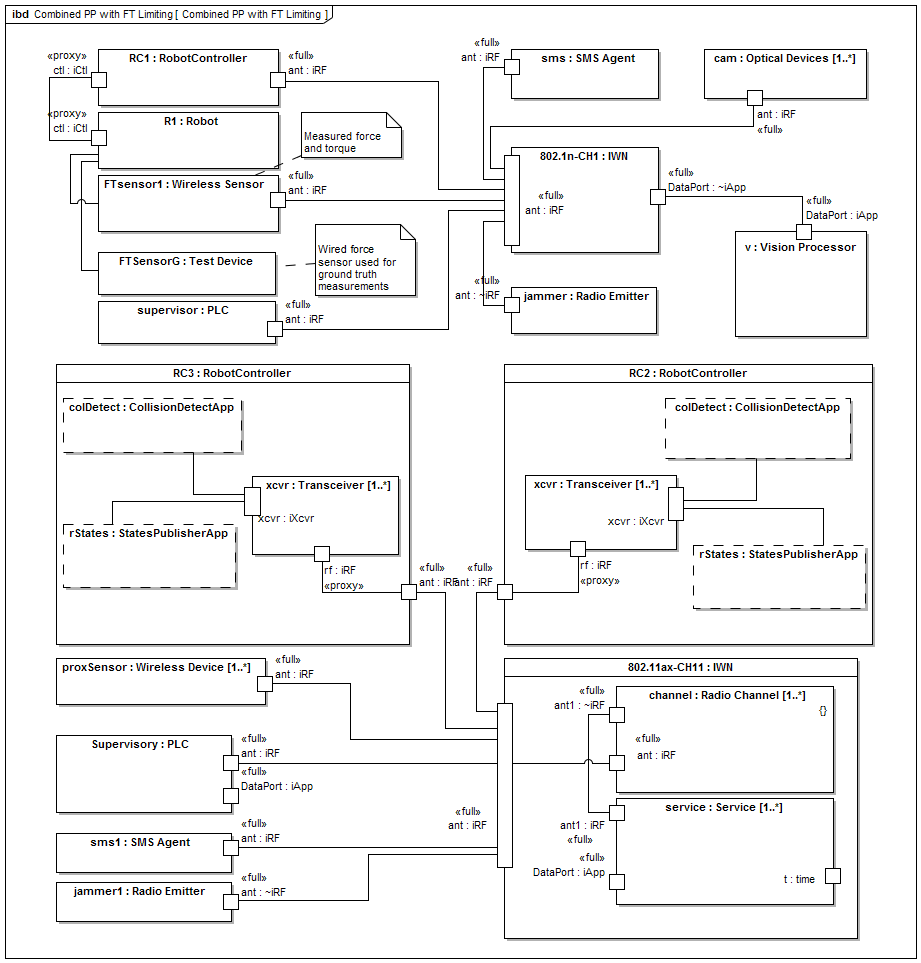
\includegraphics[width=1.05\textwidth]{diagrams/ibd__Combined_PP_with_FT_Limiting__Combined_PP_with_FT_Limiting}
	\caption{IBD of a work-cell employing multiple networks in collaborative robot operation coexisting with robot force limiting inspection station.}
	\label{fig:workcell:examples}     
\end{figure*}

In this section we present a case study of a work-cell which includes a force-torque limiter robot application and a two-robot collaborative pick and place operation.  The model for this system is depicted in Fig.~\ref{fig:workcell:examples}.  The number and type of wireless information flows will depend on the configuration of the work, the number of applications, and the places where wireless is applied. For this case study, the force limiter section is composed of a robot controller, a robot, and an FT sensor. A PLC is used for work-cell supervision, and a test device is deployed for ground truth measurement.  An SMS agent monitors the electromagnetic spectrum.  A Radio Emitter is included to model the transmission of interference.  An IEEE 802.11n network is represented in the model by an IWN block. Properties of the radio channel and services of the communication system are therefore represented. Similarly, another example is implemented in \cite{SysML.Candell2018} for a pick-and-place scenario where the model is composed of two robots, a PLC, an IWN, and an SMS Agent in addition to proximity sensors and an IEEE 802.11ax network.

Referring to these examples, typical information flows are easily identified as connections between Wireless Device blocks and the antenna port, \textit{ant}, of the IWN.  Recall that the IWN includes radio channel and services offered by the network itself.  Therefore, all wireless information flows will traverse the IWN through the \textit{ant} port.  Applications are implied and produce and consume the information according to associated constraint properties.  Information flows are generated by the interactions between actors and include the following:  

\begin{description}
	
	\item[\textbf{Robot States}] The geometry states of the robot such as position, velocity, and acceleration of each joint or end-effector. Robot states may include Cartesian or joint space readings depending on the need of other applications or the capabilities of publisher.  Robot states are usually transmitted at 30 Hz or faster~\cite{JMarvel2017}.
	
	\item[\textbf{Force Sensor Readings}] The readings from a sensor mounted on the wrist of each robot arm. These readings are typically in the format of wrenches (linear and angular forces) and are transmitted at rates from 15 Hz for monitoring applications up to 500 Hz for force limiting and control applications~\cite{onrobot}. Other sensors may produce data in the system such as proximity sensors which can generate data in the range of 1-50 Hz~\cite{DiffuseSensorSpecs} and Tactile sensors which can have information flow rates faster than 1000 Hz~\cite{TactileInternet}.
	
	\item[\textbf{Machine Health Monitoring}] Readings from sensors mounted within machinery such as mills, routers, and lathes used to sense and predict deviations of mechanical components from design tolerances. Readings for prognostics and health monitoring are often aggregated at the source with statistical metrics being communicated to a factory enterprise application; however, non-aggregated readings may also be transmitted to a remote signal analyzer.  Health monitoring sensors measure temperature, vibration, acceleration, inclination, position, and rates of change of angles. Information flows from a single aggregation point may reach 200 kB/s on average for a 6-DOF sensor apparatus described in~\cite{ELWeiss}. While the outputs of health monitoring sensors are usually wired into a local aggregation devices, it is desirable to transmit these readings to an on-line optimizer or PLC within the work-cell~\cite{Weiss2016.PHM}.
	
	\item[\textbf{IO States and Supervisory Messages}] These contain both the boolean-valued readings and commands from sensors, and task orders in the form of short commands and lists of instructions which can originate from any supervisor within the network such as a PLC or other controller. Sensor readings (inputs) and actuation commands (outputs) are transmitted in periodically or pseudo-randomly at rates indicative of movements of machinery and materials through the manufacturing process.  Typical analog and boolean IO states range from to 10 Hz to 100 Hz depending on the manufacturing process~\cite{TwinCAT}.
	% 		\item[Supervisory Messages] Directives and task orders in the form of short commands and lists of instructions and can originate from any supervisor within the network such as a PLC or other controller. Supervisory messages include state information such as task status from collaborating actors within the work-cell. 
	
	\item[\textbf{SMS Events}] The SMS agent will communicate state information and directives to controllers within the work-cell.  These messages allow the automation system to react under anomalous spectrum conditions within the work-cell. These information flows may be necessary for safe operation of the work-cell. The data rate of reports from an SMS agent without processing or compression can be in the range of 1 to 10 megabits per second (Mbps)~\cite{cuevas_2015}.
	
	\item[\textbf{Vision Applications}] The vision system will communicate videos or images for processing and decision making. Typical Video flows can have the rates of 30 Hz for surveillance and 125 Hz for motion capturing~\cite{industrialCCTV, ELWeiss}. Information flow for Object tracking systems can have the rate of 10-200 Hz depending on the tracked objects and the required accuracy~\cite{lidar, motioncapture}. 
\end{description}
%\vspace{5mm}


%     % THIS TABLE TO BE REMOVED 8/2/2018
% 	\begin{table}[tbp]
% 		\centering
% 		\caption{Work-cell information flows.}
% 		\label{tab:infoflows}
% 		\begin{threeparttable}
% 			%begin tabular
% 			% Table generated by Excel2LaTeX from sheet 'infoflows (2)'
\begin{tabular}{lccc}
\textbf{Information Flow} &
  \textbf{Information Rate (Hz)} &
  \textbf{Protocol} &
  \textbf{Citation}
  \\
\midrule
\textbf{Robotics} &
   &
    &
  
  \\
Joint states &
  30-1000 &
  Datagram &
  \cite{JMarvel2017}
  \\
Task states &
  1-5 &
  Reliable &
  TBS
  \\
End-effector commands &
  \tnote{*} &
  Reliable &
  TBS
  \\
Collision events &
  \tnote{*} &
  Reliable &
  TBS
  \\
\midrule
\textbf{Sensors} &
   &
    &
  
  \\
Force/Torque &
  15-500 &
  Datagram &
  TBS
  \\
Proximity &
  1-50 &
  Reliable &
  \cite{DiffuseSensorSpecs}
  \\
Tactile &
  $>$1000 &
  Reliable &
  \cite{TactileInternet}
  \\
\midrule
\textbf{Vision} &
   &
    &
  
  \\
Video &
  30 (Surveillance)-175 (motion capture) &
  Datagram &
  \cite{industrialCCTV, labOpticalCameraSpecs}
  \\
Tracking &
  10-100 &
  Datagram &
  \cite{LIDA15Hz}
  \\
\midrule
\textbf{Supervision} &
   &
   &
  
  \\
Command/control &
  1-5 &
  Reliable &
  TBS
  \\
IO States &
  10-100 &
  Reliable &
  \cite{TwinCAT}
  \\
\midrule
\textbf{Spectrum Monitoring} &
   &
   &
  
  \\
SMS Events &
  \tnote{*} &
  Reliable &
  TBS
  \\
SMS Reports &
  <1 &
  Reliable &
  TBS
  \\
\bottomrule
\end{tabular}%
%end tabular
% 			\begin{tablenotes}
%             	\item[] \textcolor{blue}{add information about the purpose of this table. What are the flow items, impact to bandwidth, and }
% 				\item[*] Indeterminate flow rate
% 				\item[] \textcolor{red}{need validation and citations}
% 			\end{tablenotes}
% 		\end{threeparttable}
% 	\end{table}

\section{Discussion and Conclusions}\label{sec:conclusion}
A model was developed using SysML. The developed model is constructed of the elements necessary to construct useful representations of factory work-cells in which wireless networks are used to transport information necessary for automated control system operation.  Reusable, derivable elements are developed and then extended to represent the constructs of the work-cell such as robot control, supervisory control, vision, safety, and spectrum monitoring.  An industrial wireless network is then developed and constraints of the radio channel and network services are formalized. Using the architectural model, information flows are explored and incorporated within. 

It is important to mention that this model includes an often overlooked component of any industrial wireless deployment which is the spectrum monitoring system and also considers the human-robot and robot-robot interactions in industrial environments. The current model includes various systems constraints including motion constraints, radio channel constraints, and networking constraints. The parametric constraints are provided as examples and can be replaced with executable computer code thereby making the model useful for simulation depending on the modeling tool selected. Furthermore, the applications within the robotic work-cell define many information flows requiring careful analysis to achieve reliability and latency necessary for the safety and control of the manufacturing process.

With increased dependency on wireless communications for more complex manufacturing systems, the projection of manufacturing requirements onto the wireless communication system becomes less obvious. Such analysis of this projection is essential for future research of manufacturing systems. As such, the architectural elements and information flows exposed by an abstract model
are a necessary first step. Our model in its current state of development is comprehensive enough to support architectural and ontological analyses of the factory work-cell.  As such, information about the relationships between components of a work-cell and attributes related to the wireless network may be discovered. Therefore, our model serves as a foundation for future systems engineering analyses. Moreover, our model may be used as a tool for academic and industry exploration of wireless testbed development.  We make the model openly available through GitHub at~\cite{SysML.Candell2018}.



\chapter{Industry Wireless Testbed}
paper on testbed construction; ground truth; data sources network and physical; data outputs; paper on graph database approach for organization of data
\chapter{Machine Learning Applications}
two papers on machine learning
\section{Introduction}
\section{Force Seeking Use Cases}
\section{Exploration of ML Algorithms}
\section{Results}
\section{Conclusions}
Discussion, Perspectives, restate findings


% Automatic Lettrine and Minitoc at the begining of the chapter.
%
% The following macros are formatting the text at the begining of a chapter according to the
% standard format.
%
% \chapterintro               See \chapterintrotosection.
%
% \chapterintro*              Similar to \chapterintro, except that the minitoc will be ignored.
%
% \chapterintrotosection      transform to lettrine the first letter that is following this macro
%                             until the next following \section macro.
%                             YOU MUST type the \section macro
%                             in the same file as the \chapterintrotosection macro.
%                             AND
%                             put a minitoc (if the minitoc package is included) just before
%                             the next following \section macro.
%
% \chapterintrotoinput        transform to lettrine the first letter that is following this macro
%                             until the next following \input macro.
%                             YOU MUST type the \input macro
%                             in the same file as the \chapterintrotoinput macro.
%                             AND
%                             put a minitoc (if the minitoc package is included) just before
%                             the next following \input macro.
%
% \chapterintrotoinclude      transform to lettrine the first letter that is following this macro
%                             until the next following \include macro.
%                             YOU MUST type the \include macro
%                             in the same file as the \chapterintrotoinclude macro.
%                             AND
%                             put a minitoc (if the minitoc package is included) just before
%                             the next following \include macro.

%\chapterintro*
%\chapterintro
%\chapterintrotosection
%\chapterintrotoinput
%\chapterintrotoinclude




 
%%--------------------
%% Start the end of the thesis
\backmatter
 
%%--------------------
%% Bibliography
 
%% PERSONAL BIBLIOGRAPHY (use 'multibib')
 
%% Change the style of the PERSONAL bibliography
%\bibliographystylePERSO{phdthesisapa}
 
%% Add the chapter with the PERSONAL bibliogaphy.
%% The name of the BibTeX file may be the same as
%% the one for the general bibliography.
%\bibliographyPERSO{biblio.bib}
 
%% Below, include a chapter for the GENERAL bibliography.
%% It is assumed that the standard BibTeX tool/approach
%% is used.
 
%% GENERAL BIBLIOGRAPHY
 
%% To cite one of your PERSONAL papers with the style
%% of the PERSONAL bibliography: \cite{key}
 
%% To force to show one of your PERSONAL papers into
%% the PERSONAL bibliography, even if not cited in the
%% text: \nocite{key}
 
%% The following line set the style of
%% the GENERAL bibliogaphy.
%% The "phdthesisapa" is a "apalike" style with the following
%% differences:
%% a) The titles are output with the color of the institution.
%% b) The name of the PhD thesis' author is underlined.
\bibliographystyle{phdthesisapa}
%% The following line may be used in place of the previous
%% line if you prefer "numeric" citations.
%\bibliographystyle{phdthesisnum}
 
%% Link the GENERAL bibliogaphy to a BibTeX file.
\bibliography{biblio.bib}
 
%%--------------------
%% List of figures and tables
 
%% Include a chapter with a list of all the figures.
%% In French typograhic standard, this list must be at
%% the end of the document.
\listoffigures
 
%% Include a chapter with a list of all the tables.
%% In French typograhic standard, this list must be at
%% the end of the document.
\listoftables
 
%%--------------------
%% Include a list of definitions
\listofdefinitions

%%--------------------
%% Appendixes
\appendix
\part{Annexes}
 
\chapter{Premier chapitre des annexes}

\chapter{Second chapitre des annexes}
 
\end{document}
